\documentclass[12pt, a4paper, oneside]{ctexbook}
\usepackage{amsmath, amsthm, amssymb, bm, graphicx, hyperref, mathrsfs, diagbox, color, tikz}
\usetikzlibrary{positioning, arrows.meta}

\newcommand{\Var}{\operatorname{Var}}
\newcommand{\Cov}{\operatorname{Cov}}
\newcommand{\dx}{\operatorname{dx}}
\newcommand{\dt}{\operatorname{dt}}
\newcommand{\dbx}{\operatorname{d}\mathbf{x}}
\newcommand{\dy}{\operatorname{dy}}
\newcommand{\Vol}{\operatorname{Vol}}
\newcommand{\bmu}{\bm{\mu}}
\newcommand{\bK}{\mathbf{K}}
\newcommand{\bx}{\mathbf{x}}
\newcommand{\Tr}{\text{Tr}}

\title{{\Huge{\textbf{EE142 \\ Fundamentals of Information Theory}}}\\Lecture notes}
\author{Zhou Shouchen\\ 2021533042 \\ \href{https://github.com/zsc2003/ShanghaiTech-EE142}{\LaTeX{} source code on GitHub}}
\date{\today}
\linespread{1.4}
\newtheorem{theorem}{定理}[section]
\newtheorem{definition}[theorem]{定义}
\newtheorem{lemma}[theorem]{引理}
\newtheorem{corollary}[theorem]{推论}
\newtheorem{example}[theorem]{例}
\newtheorem{proposition}[theorem]{命题}

\begin{document}

\maketitle

% -------------------- chapters --------------------
\pagenumbering{Roman}
\setcounter{page}{1}
\tableofcontents
\newpage
\setcounter{page}{1}
\pagenumbering{arabic}

\chapter{Summary}


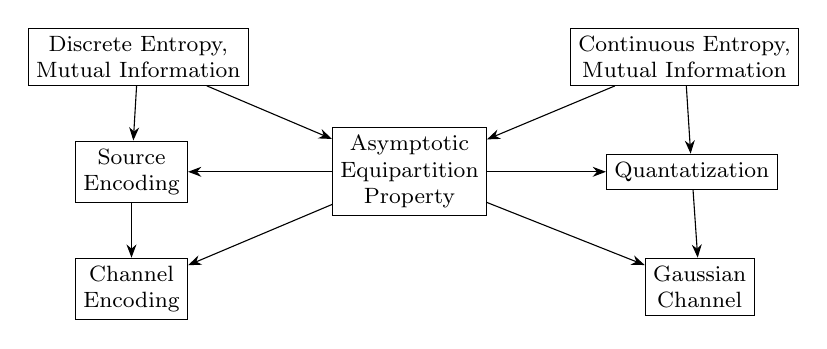
\begin{tikzpicture}[
    every node/.style={rectangle, draw, align=center},
    arrow/.style={-Stealth}
]
\centering
\footnotesize
\node (AEP) {Asymptotic \\ Equipartition \\ Property};
\node (discrete) [above left=15pt and 30pt of AEP] {Discrete Entropy, \\ Mutual Information};
\node (sourceencoding) [left=52pt of AEP] {Source \\ Encoding};
\node (channelencoding) [below left=15pt and 52pt of AEP] {Channel \\ Encoding};

\node (continuous) [above right=15pt and 30pt of AEP] {Continuous Entropy, \\ Mutual Information};
\node (quantatization) [right=43pt of AEP] {Quantatization};
\node (Gaussianchannel) [below right=15pt and 57pt of AEP] {Gaussian \\ Channel};

\draw [arrow] (discrete) -- (AEP);
\draw [arrow] (continuous) -- (AEP);
\draw [arrow] (AEP) -- (channelencoding);
\draw [arrow] (AEP) -- (sourceencoding);
\draw [arrow] (AEP) -- (Gaussianchannel);
\draw [arrow] (AEP) -- (quantatization);
\draw [arrow] (discrete) -- (sourceencoding);
\draw [arrow] (sourceencoding) -- (channelencoding);
\draw [arrow] (continuous) -- (quantatization);
\draw [arrow] (quantatization) -- (Gaussianchannel);
\end{tikzpicture}

A.E.P. 将所有的章节连接起来.

主要围绕香农三大定理展开: (注意成立的条件! 所有事情要满足其条件才行!)
\begin{enumerate}
\item Lossless Source Coding Theorem (\textcolor{red}{前提: $x^n\stackrel{i.i.d.}{\sim} p(x)$})
$$L^* = H(X)$$

\item Channel Coding Theorem (\textcolor{red}{前提: Memoryless Channel})
$$C^* = \max_{p(x)}I(X;Y)$$

\item Rate Distortion Theorem (\textcolor{red}{前提: $x^n\stackrel{i.i.d.}{\sim} p(x)$})
$$R(D) = \min_{p(x), \mathbb{E}(X)\leq p^2}I(X;\hat{X})$$
\end{enumerate}

Some interesting topics but not covered in class:
$\S 11.3$ Universal Source Coding, $\S 11.10$ Fisher Information, $\S 15.10$ General Multiterminal Networks.

$\ldots\ldots\ldots\ldots$ A lot of interesting topics $\ldots\ldots\ldots\ldots$
\chapter{Entropy, Relative Entropy, Mutual Information}
Book Chapter2. (P39)

$\log x$若无特殊说明, 默认为$\log_2 x$, $0\log 0=0$.

离散型随机变量$\mathcal{X}$看作是有限的, i.e. $|\mathcal{X}|<+\infty$.

\section{Law of Large Numbers}

几种收敛方式:
Given a sequence $X_1,X_2,\ldots,X_n$, it converges to $X$:
\begin{itemize}
\item[1.] In probability(依概率收敛):
$$\lim\limits_{n\to\infty}P\left(|X_n-X|>\epsilon\right)=0\Rightarrow\lim\limits_{n\to\infty}P\left(|X_n-X|>\epsilon\right)<\delta$$
\item[2.] In mean square(均方收敛): $\lim\limits_{n\to\infty}\mathbb{E}\left[(X_n-X)^2\right]=0$.
\item[3.] Almost surely / with probability 1: $P\left(\lim\limits_{n\to\infty}X_n=X\right)=1$.
\end{itemize}

Law of Large Numbers(LLN): 大数定律.
$x_1,\ldots,x_n\stackrel{i.i.d.}{\sim}p(x)$, then $\dfrac{1}{n}\sum\limits_{i=1}^nx_i$ converges to $\mathbb{E}[x]$.

(1) in probability: Weak LLN(Weak Law of Large Numbers).

(2) w.p. $1$: Strong LLN(Strong Law of Large Numbers).
\section{Entropy Rates of Stochastic Processes}


\begin{definition}
The \textbf{entropy rate} of a stochastic process $\{X_i\}$ is defined as
$$H\left(\mathcal{X}\right) = \lim_{n\to\infty} \frac{1}{n}H(X_1,X_2,\cdots,X_n)$$
\end{definition}
随机过程$X(t)$的不确定度为$H(X(t))$, 整个随机过程的不确定度为$H\left(\mathcal{X}\right)$. $H\left(\mathcal{X}\right)$平衡整个过程中每个变量的不确定度(信息量), 极限可能不存在(e.g. 趋于极限时$H(\mathcal{X}$)可能在振荡, 而不是收敛到具体值).但$H\left(\mathcal{X}\right)$一定有界:
$$0\leq H(X_i)\leq \log|\mathcal{X}| \Rightarrow 0\leq H\left(\mathcal{X}\right)\leq \log|\mathcal{X}|$$

\begin{example}
\begin{itemize}
\item[1.] $X_1,X_2,\cdots,X_n$ are i.i.d., then:
$$H\left(\mathcal{X}\right) = \lim_{n\to\infty} \dfrac{1}{n}H(X_1,X_2,\cdots,X_n) = \lim_{n\to\infty} \dfrac{1}{n}\sum_{i=1}^nH(X_i) = H(X_1) = \ldots = H(X_n)$$

\item[2.] $X_1\perp X_2\perp\ldots\perp X_n$, then:
$$H\left(\mathcal{X}\right)=\lim_{n\to\infty}\dfrac{1}{n}H(X_1,X_2,\cdots,X_n) = \lim_{n\to\infty}\dfrac{1}{n}\sum_{i=1}^nH(X_i)$$

\end{itemize}
\end{example}

\begin{definition}
Define a related quantity for entropy rate:
$$H'\left(\mathcal{X}\right) = \lim_{n\to\infty}H(X_n|X_{n-1},X_{n-2},\cdots,X_1)$$
\end{definition}

\begin{theorem}
For a stationary stochastic process $\{X(t)\}$, $H\left(\mathcal{X}\right)$ limit exists:
$$H\left(\mathcal{X}\right) = H'\left(\mathcal{X}\right) = \lim_{n\to\infty}H(X_n|X_{n-1},X_{n-2},\cdots,X_1)$$
\end{theorem}

\begin{example}
For a stationary Markov chain: $X_1\rightarrow X_2\rightarrow\cdots\rightarrow X_n$ \textbf{(记忆为1!)}
$$H\left(\mathcal{X}\right)=H'\left(\mathcal{X}\right)=\lim_{n\to\infty}H(X_n|X_{n-1},\ldots,X_1)=H(X_n|X_{n-1})=\ldots=H(X_2|X_1)$$
\end{example}
\section{Fano's Inequality, Channel Coding Theorem(Shannon's Second Theorem)}
简单理解: 从jointly typical set的角度. 在第四章的最后(jointly AEP), 每个$X^n$平均会有$\frac{2^{nH(X,Y)}}{2^{nH(X)}}=2^{nH(Y|X)}$个$Y^n$与之jointly typical, 即将所有的$Y^n$进行划分, 每份的大小为$2^{nH(Y|X)}$, 可以分成 $\frac{2^{nH(Y)}}{2^{nH(Y|X)}}=2^{nI(X;Y)}$份. 这样平均每次用信道发送的bit数为$\frac{2^{nI(X;Y)}}{n}=I(X;Y)$

在保证无损传输的情况下, 信道容量:
$$C\triangleq\max R=\max\limits_{p(x)}I(X;Y)$$

\begin{definition}
Channel Coding Theorem(Shannon's Second Theorem) \\
对于一个rate 为 $R$ 的DMC, 只要$R<C$, 那么这个DMC是 \textcolor{blue}{achievable} 的. i.e. $\forall R<C, \exists$ a sequence of $\left(2^{nR},n\right)$ codes, 使得最大错误概率$\lambda^{(n)}\to 0$. \\
\textcolor{blue}{Conversely}, 任意sequence of $\left(2^{nR},n\right)$ codes, $\lambda^{(n)}\to 0$, 那么$R\leq C$.
\end{definition}
所以证明需要从两个角度: \\
1. 可达性证明(\textcolor{blue}{achievable} proof): $\forall R<C$, $\exists (R,n)$, s.t. $\lambda^{(n)}\to 0$, 找到一种达到$C$的方法. \\
2. \textcolor{blue}{converse} proof: 所有方法都不可能超过$C$. i.e. $R>C$时, $p_e^{(n)}\to 1 \Rightarrow R\leq C$时, $p_e^{(n)}\not\to 0$.


\textcolor{blue}{1. 可达性证明 achievable proof}:

<1>. 码本构建(randomly coding): fixed $p(x)$, 产生$2^{nR}$个长度为$n$的codewords: $X^n(1),\ldots,X^n(2^{nR})\stackrel{i.i.d.}{\sim}p(X^n)=\prod\limits_{i=1}^np(x_i)$.
\begin{figure}[htbp]
    \centering
    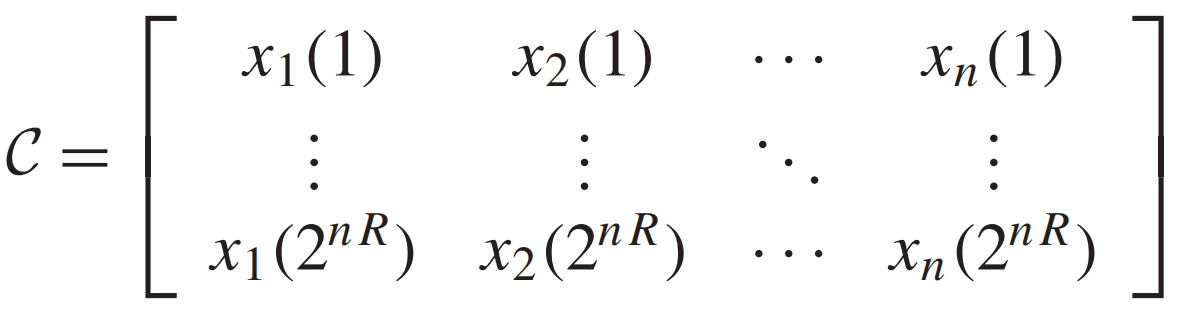
\includegraphics[width=0.5\textwidth]{./figures/chapter5/codebook.png}
\end{figure}

$X_i(w)$表示第$w$个codeword的第$i$个bit(下标为$i$). \\
码本构建好之后发给发送端和接收端(is known by the encoder and the decoder). 同时, 认为sender和receiver知道channel transition matrix $p(y|x)$.

<2>. Encoder: 随机生成一个数字 $w$, $p(W=w)=\dfrac{1}{2^{nR}}$, 从codebook $\mathcal{C}$中找出第$w$行$X^n(w)$, 发到信道当中.

<3> Decoder: reciver 接收由 $p(y^n|x^n(w))=\prod\limits_{i=1}^np(y_i|x_i(w))$ 生成的 $y^n$, 从codebook中找出一条message $\hat{W}$, s.t. $(X^n(\hat{W}), y^n)\in A_{\epsilon}^{(n)}(P_{X,Y})$, 且 no other index $W'\neq \hat{W}$ s.t. $(X^n(W'), y^n)\in A_{\epsilon}^{(n)}(P_{X,Y})$.

若找不到$\hat{W}$, an error is decleared.

<4> Error probability analysis: \\
先忽略码本的随机性 ($p(\mathcal{C})=\prod\limits_{w}^{2^{nR}}\prod\limits_{i=1}^np(x_i)(w)$), 考虑单一码本的情况. \\
发生错误: $\mathcal{E}=\left\{\hat{W}(Y^n) \neq W\right\}$. \\
考虑定义: $\lambda(i)=\Pr\left[\hat{W}\neq i|W=i\right]$, 则 $\Pr\left[\mathcal{E}|W=i\right]=\lambda(i)$. \\
$\Rightarrow \Pr\left[\hat{W}\neq W\right]=\sum\limits_{w=1}^{2^{nR}}p(W=w)\lambda(w)=\sum\limits_{w=1}^{2^{nR}}\dfrac{1}{2^{nR}}\lambda(w)$.

由于$W=1,\ldots,2^{nR}$是等概率产生的, 且地位相同, 所以 W.L.O.G. 取 $W=1$时的情况进行分析:

定义事件 $E_i=\left\{\left(X^{n}(i),Y^n\right)\in A_{\epsilon}^{(n)}(P_{X,Y})\right\}$, i.e. the i-th codeword is joint typical with the received sequence $Y^n$. \\
由jointly AEP, we can get that for sufficiently large $n$:
$$\Pr\left[E_1^c:\left(X^{n}(i),Y^n\right)\not\in A_{\epsilon}^{(n)}(P_{X,Y}) \right]\to 0 \Rightarrow \Pr\left[E_1^c: \left(X^{n}(i),Y^n\right)\not\in A_{\epsilon}^{(n)}(P_{X,Y})\right]\leq \epsilon$$
由于生成codebook $\mathcal{C}$时, 每一行的产生是独立的, i.e. $X^n(1)$与$X^n(2),\ldots,X^n(2^{nR})$是独立的, 所以$Y^n$与$X^n(i)$也是独立的, 所以有:
$$\Pr\left[E_i:\left(X^{n}(i),Y^n\right)\in A_{\epsilon}^{(n)}(P_{X,Y}) \right]\leq 2^{-n\left(I(X;Y)-3\epsilon\right)}$$
由jointly AEP, 当$R<I(X;Y)-3\epsilon$时
\begin{align*}
\Pr\left[\hat{W}\neq 1|W=1\right] &= \Pr\left[E_1^c\cup E_2\cup\ldots\cup E_{2^{nR}}\right] \\
&\leq \Pr\left[E_1^c\right] + \sum\limits_{w=2}^{2^{nR}}\Pr\left[E_w\right] \\
&\leq \epsilon + (2^{nR}-1) 2^{-n\left(I(X;Y)-3\epsilon\right)} \\
&\leq \epsilon + 2^{n\left(R-I(X;Y)+3\epsilon\right)} \\
&\leq 2\epsilon \quad \text{(sufficiently large $n$, $R<I(X;Y)-3\epsilon\Rightarrow 2^{n\left(R-I(X;Y)+3\epsilon\right)}\to 0<\epsilon$)}
\end{align*}
总结: 选择证明中取等时的分布作为真实分布 $p(x)\gets p^*(x)$, 此时$\forall R<I(X;Y)-3\epsilon$, i.e. $R<C$, 错误概率$p_e^{(n)}=\Pr\left[\hat{W}\neq W\right]\to 0\Rightarrow \lambda^{(n)}\to 0$. (Actually, $\lambda^{(n)}$条件比$p_e^{(n)}$更强, 但是$p_e^{(n)}$更容易计算)

若将codebook $\mathcal{C}$ 的随机性也考虑进去, 则会得到更加平均的结果:
$$\Pr\left[\hat{W}\neq W\right]=\sum_{w=1}^{2^{nR}}\sum_{\mathcal{C}}\Pr[\mathcal{C}]\dfrac{1}{2^{nR}}\lambda_w(\mathcal{C})=\lambda_1(\mathcal{C})\Rightarrow \Pr(\mathcal{E}|\mathcal{C}^*)\leq 2\epsilon$$
The best codebook $\mathcal{C}^*$ 中必然由超过一半的indices $i$ and their assciated codewords $X^n(i)$, 满足 $\lambda_i\leq 4\epsilon$, 否则$\Pr(\mathcal{E}|\mathcal{C}^*)>2\epsilon$. 砍去另一半codewords, 可以得到rate为$R'=\dfrac{\frac{2^{nR}}{2}}{n}=R-\dfrac{1}{n}$, s.t. $\lambda^{(n)}\leq 4\epsilon\to 0$. 所以可以使得 $\epsilon$ 不断的取小, 说明了$R$可以取到$C$的任意接近的地方.(取$p^*(x)$时, $C=I(X;Y), R=I(X;Y)-3\epsilon\to C$)

由此证明了 Achievability.

\begin{proposition}
Zero-error codes.
$$p_e^{(n)}\to 0 \Rightarrow R\leq C$$
\end{proposition}
proof: \\
Channel encoding 满足Markov chain $W\to X^n(W)\to Y^n\to \hat{W}$, so from data-processing inequality:
$$I(W; Y^n)\leq I(X^n(W); Y^n)$$

由 DMC的 memoryless, i.e. $p(Y_i|Y_1,\ldots,Y_{i-1},X^n)=p(Y_i|X_i)$, so
\begin{align*}
I(X^n;Y^n) &= H(Y^n) - H(Y^n|X^n) \\
&= \sum_{i=1}^nH(Y_i|Y_1,\ldots,Y_{i-1}) - \sum_{i=1}^nH(Y_i|Y_1,\ldots,Y_{i-1}, X^n) \\
&\leq \sum_{i=1}^nH(Y_i) - \sum_{i=1}^nH(Y_i|X_i) \qquad \text{(memoryless \& conditioning reduced entropy)} \\
&= \sum_{i=1}^n I(X_i;Y_i) \\
&\leq nC \qquad\qquad\qquad\qquad\qquad\quad\ \ \text{($Y_i$ are independent, $p_i(x)=p^*(x)$)}
\end{align*}

Since the channel is zero-error, so $\hat{W}=g(Y^n)=W$, i.e. $H(W|Y^n)=0$.
\begin{align*}
nR &= H(W) \\
&= H(W|Y^n) + I(W;Y^n) \\
&= I(W;Y^n) \qquad\quad\ \text{($H(W|Y^n)=0$)} \\
&\leq I(X^n;Y^n) \qquad\quad \text{(data-processing inequality)} \\
&\leq nC
\end{align*}

So for any zero-error $\left(2^{nR}, n\right)$ code, for all $n$:
$$R\leq C$$

\textcolor{blue}{2. converse proof: 证明$R>C$时, $p_e^{(n)}\to 1$ or $p_e^{(n)}\not\to 0$ as $n\to\infty$.}

\begin{definition}
Fano's Inequality: 是关于$p_e$的函数, 建立条件熵和错误概率$p_e$的关系. \\
For any estimator $\hat{X}$ such that $X\to Y\to \hat{X}$, $p_e=P(\hat{X}\neq X)$, then
$$H(p_e)+p_e\log\left|\mathcal{X}\right|\geq H(X|\hat{X})\geq H(X|Y)$$
It could be weakened to:
$$1+p_e\log\left|\mathcal{X}\right|\geq H(X|\hat{X})\geq H(X|Y)$$
or
$$p_e\geq \frac{H(X|Y)-1}{\log\left|\mathcal{X}\right|}$$
\end{definition}

Proof: \\
Let $E$ be the auxiliary variable indicate where the prediction is correct. i.e.
$$E=\begin{cases}
    1, & \text{if } \hat{X}\neq X \\
    0, & \text{if } \hat{X}=X
\end{cases}$$
Then we have $p(E=1)=p_e$, so
\begin{align*}
H\left(E,X|\hat{X}\right) &= \underbrace{H\left(E|\hat{X}\right)}_{\leq H(p_e)}+\underbrace{H\left(X|E,\hat{X}\right)}_{\leq p_e\log\left|\mathcal{X}\right|} \\
&= H\left(X|\hat{X}\right)+\underbrace{H\left(E|X,\hat{X}\right)}_{=0}
\end{align*}
其中由于$E=\mathbb{I}_{X=\hat{X}}$, 所以$H\left(E|X,\hat{X}\right)=0$. \\
由于conditioning reduces entropy, 所以 $H\left(E|\hat{X}\right)\leq H(E)=H(p_e)$. \\
同时有当$E=1$时, 给定$\hat{X}$, $X$的取值共有$\left|\mathcal{X}\right|-1$种, 所以有:
\begin{align*}
H\left(X|E, \hat{X}\right) &= \sum_{e=0,1}H\left(X|E=e, \hat{X}\right)P(E=e) \\
&\leq p_e\log\left(\left|\mathcal{X}\right|-1\right) + (1-p_e)\cdot 0 \\
&\leq p_e\log\left|\mathcal{X}\right|
\end{align*}
综上, 可以得到 Fano's Inequality:
$$H(p_e)+p_e\log\left|\mathcal{X}\right|\geq H(X|\hat{X})$$
weakened to的版本可由$H\left(p_e\right)\leq 1$, 以及数据处理不等式得到:
$$I(X;Y)\geq I(X;\hat{X})\Rightarrow H(X)-H(X|Y)\geq H(X)-H(X|\hat{X})\Rightarrow H(X|\hat{X})\geq H(X|Y)$$

由于 Channel encoding 满足Markov chain $W\to X^n(W)\to Y^n\to \hat{W}$, 所以应用Fano's Inequality:
$$H(W|\hat{W})\leq H(p_e^{(n)})+p_e^{(n)}\log\left|\mathcal{W}\right|$$
其中$\mathcal{W}=\left\{1,\ldots,2^{nR}\right\}$, 所以 $\left|\mathcal{W}\right|=2^{nR}\Rightarrow \log\left|\mathcal{W}\right|=nR$, 由于$W$是等概率产生的, 所以$H(W)= \log\left|\mathcal{W}\right| = nR$. 所以有
\begin{align*}
nR &= H(W) \\
&= H(W|\hat{W}) + I(W;\hat{W}) \qquad\qquad\quad \text{(definition of mutual information)} \\
&\leq H(p_e^{(n)})+p_e^{(n)} nR + I(W;\hat{W}) \qquad \text{(Fano's Inequality)} \\
&\leq 1 + p_e^{(n)}nR + nC \qquad \text{($I(W;\hat{W})\leq I(X^n;Y^n)\leq nC$ proved in zero-error code part)} \\
\Rightarrow R &\leq \dfrac{1}{n} + p_e^{(n)}R + C \\
\Rightarrow p_e^{(n)} &\geq 1 - \dfrac{C}{R} - \dfrac{1}{nR}
\end{align*}

取等条件: $W,\hat{W}$ 无信息丢失(zero-error code), i.e. $X^n=f(W), Y^n=g(X^n)$是$W$的充分统计量, $W$到$\hat{W}$是一对一的映射. 由充分统计量(s.s.), 此时可以看作构成 Markov Chain:
\begin{align*}
W \to X^n \to Y^n \to \hat{W} \\
W \to \hat{W} \to X^n \to Y^n
\end{align*}

由于我们的前提假设是 $R>C$, 且 $R,C$ 为常数, 所以 $\dfrac{C}{R}<1$, 是常数. 当$n\to\infty$时, $\dfrac{1}{nR}\to 0<\epsilon$, 所以 $p_e^{(n)}\geq 1-\text{(constant less than $1$)} - \epsilon \not\to 0$.

所以我们证明了 $\forall R>C, p_e^{(n)}\not\to 0$, 即证明了converse proof.
\section{Sufficient Statistics}
Background: $X_1,\cdots,X_n\sim \left\{f_{\theta}(X)\right\}=\left\{\mathcal{N}(\theta,1)\right\}$(a family of distribution, 一族元素), try to estimate the unknown parameter $\theta$s with the samples $X_1,\cdots,X_n$.

用MLE估计$\theta$时, 我们知道:
$$\hat{\theta} = \dfrac{\sum\limits_{i=1}^n X_i}{n}$$
所以拥有全部样本$X_1,\cdots,X_n$, 以及$T(X_1,\cdots,X_n)=\dfrac{\sum\limits_{i=1}^n X_i}{n}$, 对于预测$\theta$的效果是相同的$\Rightarrow$ 大大减少了数据储存量.

两者对参数的估计效果相同: $T(X_1,\cdots,X_n)$对变量的操作没有信息损失!

\begin{definition}
$T(X_1,\cdots,X_n)$ is the sufficient statistic(s.s.), if the Markov chain holds:
$$\theta\leftrightarrow T\left(X_1,\cdots,X_n\right)\leftrightarrow \left(X_1,\cdots,X_n\right)$$
\end{definition}
由于$X\leftrightarrow Y\leftrightarrow g(Y)$天然成立, 所以$$\theta\leftrightarrow \left(X_1,\cdots,X_n\right) \leftrightarrow T\left(X_1,\cdots,X_n\right)$$
From the data processing Inequality, we have:
\begin{align*}
I\left(\theta;T\left(X_1,\cdots,X_n\right)\right) &\geq I\left(\theta;\left(X_1,\cdots,X_n\right)\right) \\
I\left(\theta;\left(X_1,\cdots,X_n\right)\right) &\geq I\left(\theta;T\left(X_1,\cdots,X_n\right)\right) \\
\textcolor{red}{I\left(\theta;\left(X_1,\cdots,X_n\right)\right)} &\textcolor{red}{= I\left(\theta;T\left(X_1,\cdots,X_n\right)\right)}
\end{align*}

\begin{example}
$X_1,\cdots,X_n \stackrel{i.i.d.}{\sim} Bern(\theta)$, $n$ is known.
The sufficient statistic is
$$T(X_1,\cdots,X_n)=\sum_{i=1}^n X_i$$
prove:
$$P\left[(X_1,\cdots,X_n)=(x_1,\cdots,x_n)\big|\sum_{i=1}^nX_i=k\right]=\dfrac{1}{\binom{n}{k}}$$
与$\theta$无关, 所以$T(X_1,\cdots,X_n)$是充分统计量.
\end{example}

\begin{example}
$X_1,\cdots,X_n \stackrel{i.i.d.}{\sim} \mathcal{N}(\mu,\sigma^2)$.
$$\mu\leftrightarrow \text{样本均值} \leftrightarrow \left(X_1,\cdots,X_n\right)$$
$$\sigma\leftrightarrow \text{样本方差} \leftrightarrow \left(X_1,\cdots,X_n\right)$$
\end{example}

\begin{example}
$f_{\theta}=Unif(\theta,\theta+1)$\\
$T(X_1,\cdots,X_n)=\left\{\min\left\{X_1,\cdots,X_n\right\},\max\left\{X_1,\cdots,X_n\right\}\right\}$

simply prove:
Since $X_1, \ldots, X_n\stackrel{i.i.d}{\sim}\operatorname{Unif}(\theta, \theta+1)$, so the PDF:
$$f\left(x_i \mid \theta\right)= \mathbb{I}_{\theta\leq x_i \leq \theta+1}$$
The joint distribution is:
$$f\left(x_1, \ldots, x_n \mid \theta\right) = \prod_{i=1}^n f\left(x_i \mid \theta\right) = \mathbb{I}_{\theta \leq \min \left\{x_1, \ldots, x_n\right\} \& \max \left\{x_1, \ldots, x_n\right\} \leq \theta+1}$$
when $\theta \leq \min \left\{x_1, \ldots, x_n\right\}, \left\{x_1, \ldots, x_n\right\} \leq \theta+1$, $g\left(T\left(x_1, \ldots, x_n\right), \theta\right)=1$. \\
So $T(X)=\left\{\min \left\{X_1, \ldots, X_n\right\}, \max \left\{X_1, \ldots, X_n\right\}\right\}$ is a sufficient statistic.

\end{example}

\begin{proposition}
充分统计量可能不唯一. e.g. $\forall k$
\begin{align*}
\theta &\leftrightarrow X \leftrightarrow X+k \\
\theta &\leftrightarrow X+k \leftrightarrow X
\end{align*}
\end{proposition}

\begin{definition}
所以引入最小充分统计量(minimal sufficient statistic):
$T(X)$ is the minimal sufficient statistic, if for any other sufficient statistic $U(X)$ has:
$$\theta\leftrightarrow T(X)\leftrightarrow U(X)\leftrightarrow X$$
\begin{figure}[htbp]
    \centering
    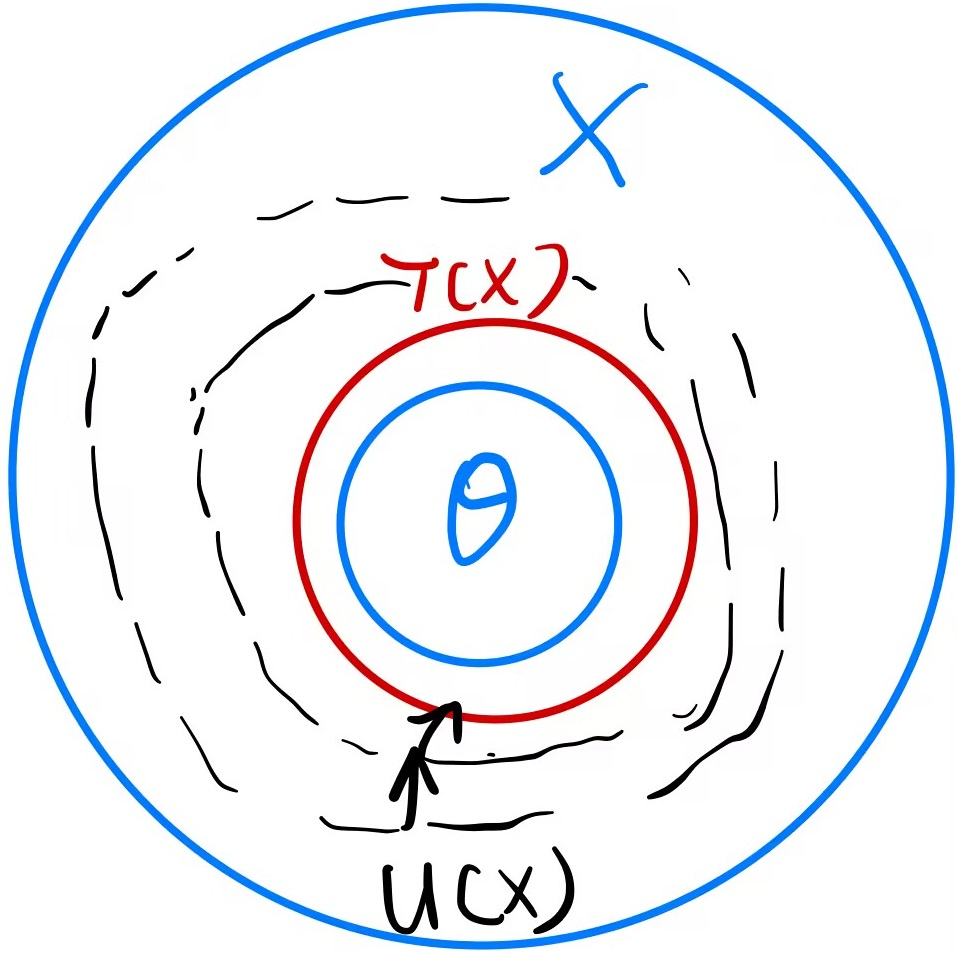
\includegraphics[width=0.41\textwidth]{./figures/chapter1/minimum_sufficient_statistic.png}
\end{figure}
\end{definition}

\begin{proposition}
$T(X),U(X)$ are the sufficient statistic, so
\begin{align*}
I(\theta;T(X)) &= I(\theta;X) \\
I(\theta;U(X)) &= I(\theta;X)
\end{align*}
$T(X)$ is the minimal sufficient statistic, so from data processing inequality:
$$I(X;T(X))\leq I(X;U(X))$$
understanding: 从上面的关系图来看, $T(X)$是对$U(X)$进行不断提纯,仅可能的去掉和$X$相关的信息, 只保留和$\theta$相关的信息.

e.g. 图像分类, 最理想的情况下, $(X,Y)$ 的最小充分统计量是$T(X)=Y$.
\end{proposition}
\section{Law of Large Numbers}

几种收敛方式:
Given a sequence $X_1,X_2,\ldots,X_n$, it converges to $X$:
\begin{itemize}
\item[1.] In probability(依概率收敛):
$$\lim\limits_{n\to\infty}P\left(|X_n-X|>\epsilon\right)=0\Rightarrow\lim\limits_{n\to\infty}P\left(|X_n-X|>\epsilon\right)<\delta$$
\item[2.] In mean square(均方收敛): $\lim\limits_{n\to\infty}\mathbb{E}\left[(X_n-X)^2\right]=0$.
\item[3.] Almost surely / with probability 1: $P\left(\lim\limits_{n\to\infty}X_n=X\right)=1$.
\end{itemize}

Law of Large Numbers(LLN): 大数定律.
$x_1,\ldots,x_n\stackrel{i.i.d.}{\sim}p(x)$, then $\dfrac{1}{n}\sum\limits_{i=1}^nx_i$ converges to $\mathbb{E}[x]$.

(1) in probability: Weak LLN(Weak Law of Large Numbers).

(2) w.p. $1$: Strong LLN(Strong Law of Large Numbers).

% \chapter{.}


% \section{.}


% \theorem
% \definition
% \lemma
% \corollary
% \example
% \proposition
\chapter{Data Compression}

Book Chapter5. (P129)

\section{Law of Large Numbers}

几种收敛方式:
Given a sequence $X_1,X_2,\ldots,X_n$, it converges to $X$:
\begin{itemize}
\item[1.] In probability(依概率收敛):
$$\lim\limits_{n\to\infty}P\left(|X_n-X|>\epsilon\right)=0\Rightarrow\lim\limits_{n\to\infty}P\left(|X_n-X|>\epsilon\right)<\delta$$
\item[2.] In mean square(均方收敛): $\lim\limits_{n\to\infty}\mathbb{E}\left[(X_n-X)^2\right]=0$.
\item[3.] Almost surely / with probability 1: $P\left(\lim\limits_{n\to\infty}X_n=X\right)=1$.
\end{itemize}

Law of Large Numbers(LLN): 大数定律.
$x_1,\ldots,x_n\stackrel{i.i.d.}{\sim}p(x)$, then $\dfrac{1}{n}\sum\limits_{i=1}^nx_i$ converges to $\mathbb{E}[x]$.

(1) in probability: Weak LLN(Weak Law of Large Numbers).

(2) w.p. $1$: Strong LLN(Strong Law of Large Numbers).
\section{Entropy Rates of Stochastic Processes}


\begin{definition}
The \textbf{entropy rate} of a stochastic process $\{X_i\}$ is defined as
$$H\left(\mathcal{X}\right) = \lim_{n\to\infty} \frac{1}{n}H(X_1,X_2,\cdots,X_n)$$
\end{definition}
随机过程$X(t)$的不确定度为$H(X(t))$, 整个随机过程的不确定度为$H\left(\mathcal{X}\right)$. $H\left(\mathcal{X}\right)$平衡整个过程中每个变量的不确定度(信息量), 极限可能不存在(e.g. 趋于极限时$H(\mathcal{X}$)可能在振荡, 而不是收敛到具体值).但$H\left(\mathcal{X}\right)$一定有界:
$$0\leq H(X_i)\leq \log|\mathcal{X}| \Rightarrow 0\leq H\left(\mathcal{X}\right)\leq \log|\mathcal{X}|$$

\begin{example}
\begin{itemize}
\item[1.] $X_1,X_2,\cdots,X_n$ are i.i.d., then:
$$H\left(\mathcal{X}\right) = \lim_{n\to\infty} \dfrac{1}{n}H(X_1,X_2,\cdots,X_n) = \lim_{n\to\infty} \dfrac{1}{n}\sum_{i=1}^nH(X_i) = H(X_1) = \ldots = H(X_n)$$

\item[2.] $X_1\perp X_2\perp\ldots\perp X_n$, then:
$$H\left(\mathcal{X}\right)=\lim_{n\to\infty}\dfrac{1}{n}H(X_1,X_2,\cdots,X_n) = \lim_{n\to\infty}\dfrac{1}{n}\sum_{i=1}^nH(X_i)$$

\end{itemize}
\end{example}

\begin{definition}
Define a related quantity for entropy rate:
$$H'\left(\mathcal{X}\right) = \lim_{n\to\infty}H(X_n|X_{n-1},X_{n-2},\cdots,X_1)$$
\end{definition}

\begin{theorem}
For a stationary stochastic process $\{X(t)\}$, $H\left(\mathcal{X}\right)$ limit exists:
$$H\left(\mathcal{X}\right) = H'\left(\mathcal{X}\right) = \lim_{n\to\infty}H(X_n|X_{n-1},X_{n-2},\cdots,X_1)$$
\end{theorem}

\begin{example}
For a stationary Markov chain: $X_1\rightarrow X_2\rightarrow\cdots\rightarrow X_n$ \textbf{(记忆为1!)}
$$H\left(\mathcal{X}\right)=H'\left(\mathcal{X}\right)=\lim_{n\to\infty}H(X_n|X_{n-1},\ldots,X_1)=H(X_n|X_{n-1})=\ldots=H(X_2|X_1)$$
\end{example}
\section{Fano's Inequality, Channel Coding Theorem(Shannon's Second Theorem)}
简单理解: 从jointly typical set的角度. 在第四章的最后(jointly AEP), 每个$X^n$平均会有$\frac{2^{nH(X,Y)}}{2^{nH(X)}}=2^{nH(Y|X)}$个$Y^n$与之jointly typical, 即将所有的$Y^n$进行划分, 每份的大小为$2^{nH(Y|X)}$, 可以分成 $\frac{2^{nH(Y)}}{2^{nH(Y|X)}}=2^{nI(X;Y)}$份. 这样平均每次用信道发送的bit数为$\frac{2^{nI(X;Y)}}{n}=I(X;Y)$

在保证无损传输的情况下, 信道容量:
$$C\triangleq\max R=\max\limits_{p(x)}I(X;Y)$$

\begin{definition}
Channel Coding Theorem(Shannon's Second Theorem) \\
对于一个rate 为 $R$ 的DMC, 只要$R<C$, 那么这个DMC是 \textcolor{blue}{achievable} 的. i.e. $\forall R<C, \exists$ a sequence of $\left(2^{nR},n\right)$ codes, 使得最大错误概率$\lambda^{(n)}\to 0$. \\
\textcolor{blue}{Conversely}, 任意sequence of $\left(2^{nR},n\right)$ codes, $\lambda^{(n)}\to 0$, 那么$R\leq C$.
\end{definition}
所以证明需要从两个角度: \\
1. 可达性证明(\textcolor{blue}{achievable} proof): $\forall R<C$, $\exists (R,n)$, s.t. $\lambda^{(n)}\to 0$, 找到一种达到$C$的方法. \\
2. \textcolor{blue}{converse} proof: 所有方法都不可能超过$C$. i.e. $R>C$时, $p_e^{(n)}\to 1 \Rightarrow R\leq C$时, $p_e^{(n)}\not\to 0$.


\textcolor{blue}{1. 可达性证明 achievable proof}:

<1>. 码本构建(randomly coding): fixed $p(x)$, 产生$2^{nR}$个长度为$n$的codewords: $X^n(1),\ldots,X^n(2^{nR})\stackrel{i.i.d.}{\sim}p(X^n)=\prod\limits_{i=1}^np(x_i)$.
\begin{figure}[htbp]
    \centering
    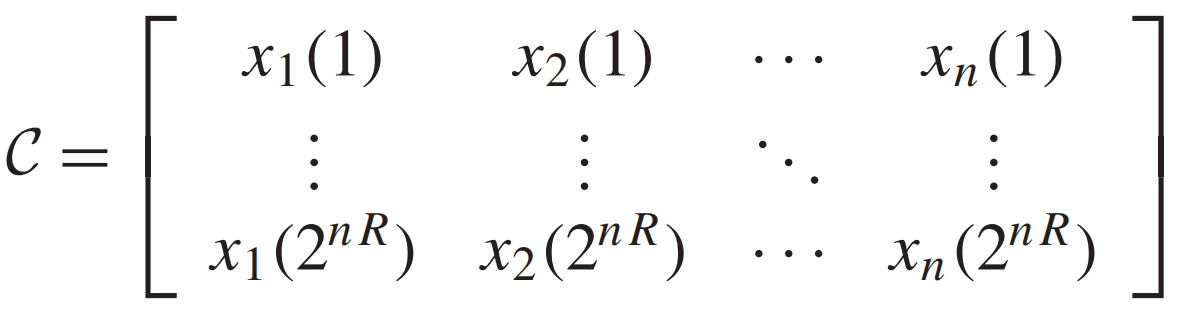
\includegraphics[width=0.5\textwidth]{./figures/chapter5/codebook.png}
\end{figure}

$X_i(w)$表示第$w$个codeword的第$i$个bit(下标为$i$). \\
码本构建好之后发给发送端和接收端(is known by the encoder and the decoder). 同时, 认为sender和receiver知道channel transition matrix $p(y|x)$.

<2>. Encoder: 随机生成一个数字 $w$, $p(W=w)=\dfrac{1}{2^{nR}}$, 从codebook $\mathcal{C}$中找出第$w$行$X^n(w)$, 发到信道当中.

<3> Decoder: reciver 接收由 $p(y^n|x^n(w))=\prod\limits_{i=1}^np(y_i|x_i(w))$ 生成的 $y^n$, 从codebook中找出一条message $\hat{W}$, s.t. $(X^n(\hat{W}), y^n)\in A_{\epsilon}^{(n)}(P_{X,Y})$, 且 no other index $W'\neq \hat{W}$ s.t. $(X^n(W'), y^n)\in A_{\epsilon}^{(n)}(P_{X,Y})$.

若找不到$\hat{W}$, an error is decleared.

<4> Error probability analysis: \\
先忽略码本的随机性 ($p(\mathcal{C})=\prod\limits_{w}^{2^{nR}}\prod\limits_{i=1}^np(x_i)(w)$), 考虑单一码本的情况. \\
发生错误: $\mathcal{E}=\left\{\hat{W}(Y^n) \neq W\right\}$. \\
考虑定义: $\lambda(i)=\Pr\left[\hat{W}\neq i|W=i\right]$, 则 $\Pr\left[\mathcal{E}|W=i\right]=\lambda(i)$. \\
$\Rightarrow \Pr\left[\hat{W}\neq W\right]=\sum\limits_{w=1}^{2^{nR}}p(W=w)\lambda(w)=\sum\limits_{w=1}^{2^{nR}}\dfrac{1}{2^{nR}}\lambda(w)$.

由于$W=1,\ldots,2^{nR}$是等概率产生的, 且地位相同, 所以 W.L.O.G. 取 $W=1$时的情况进行分析:

定义事件 $E_i=\left\{\left(X^{n}(i),Y^n\right)\in A_{\epsilon}^{(n)}(P_{X,Y})\right\}$, i.e. the i-th codeword is joint typical with the received sequence $Y^n$. \\
由jointly AEP, we can get that for sufficiently large $n$:
$$\Pr\left[E_1^c:\left(X^{n}(i),Y^n\right)\not\in A_{\epsilon}^{(n)}(P_{X,Y}) \right]\to 0 \Rightarrow \Pr\left[E_1^c: \left(X^{n}(i),Y^n\right)\not\in A_{\epsilon}^{(n)}(P_{X,Y})\right]\leq \epsilon$$
由于生成codebook $\mathcal{C}$时, 每一行的产生是独立的, i.e. $X^n(1)$与$X^n(2),\ldots,X^n(2^{nR})$是独立的, 所以$Y^n$与$X^n(i)$也是独立的, 所以有:
$$\Pr\left[E_i:\left(X^{n}(i),Y^n\right)\in A_{\epsilon}^{(n)}(P_{X,Y}) \right]\leq 2^{-n\left(I(X;Y)-3\epsilon\right)}$$
由jointly AEP, 当$R<I(X;Y)-3\epsilon$时
\begin{align*}
\Pr\left[\hat{W}\neq 1|W=1\right] &= \Pr\left[E_1^c\cup E_2\cup\ldots\cup E_{2^{nR}}\right] \\
&\leq \Pr\left[E_1^c\right] + \sum\limits_{w=2}^{2^{nR}}\Pr\left[E_w\right] \\
&\leq \epsilon + (2^{nR}-1) 2^{-n\left(I(X;Y)-3\epsilon\right)} \\
&\leq \epsilon + 2^{n\left(R-I(X;Y)+3\epsilon\right)} \\
&\leq 2\epsilon \quad \text{(sufficiently large $n$, $R<I(X;Y)-3\epsilon\Rightarrow 2^{n\left(R-I(X;Y)+3\epsilon\right)}\to 0<\epsilon$)}
\end{align*}
总结: 选择证明中取等时的分布作为真实分布 $p(x)\gets p^*(x)$, 此时$\forall R<I(X;Y)-3\epsilon$, i.e. $R<C$, 错误概率$p_e^{(n)}=\Pr\left[\hat{W}\neq W\right]\to 0\Rightarrow \lambda^{(n)}\to 0$. (Actually, $\lambda^{(n)}$条件比$p_e^{(n)}$更强, 但是$p_e^{(n)}$更容易计算)

若将codebook $\mathcal{C}$ 的随机性也考虑进去, 则会得到更加平均的结果:
$$\Pr\left[\hat{W}\neq W\right]=\sum_{w=1}^{2^{nR}}\sum_{\mathcal{C}}\Pr[\mathcal{C}]\dfrac{1}{2^{nR}}\lambda_w(\mathcal{C})=\lambda_1(\mathcal{C})\Rightarrow \Pr(\mathcal{E}|\mathcal{C}^*)\leq 2\epsilon$$
The best codebook $\mathcal{C}^*$ 中必然由超过一半的indices $i$ and their assciated codewords $X^n(i)$, 满足 $\lambda_i\leq 4\epsilon$, 否则$\Pr(\mathcal{E}|\mathcal{C}^*)>2\epsilon$. 砍去另一半codewords, 可以得到rate为$R'=\dfrac{\frac{2^{nR}}{2}}{n}=R-\dfrac{1}{n}$, s.t. $\lambda^{(n)}\leq 4\epsilon\to 0$. 所以可以使得 $\epsilon$ 不断的取小, 说明了$R$可以取到$C$的任意接近的地方.(取$p^*(x)$时, $C=I(X;Y), R=I(X;Y)-3\epsilon\to C$)

由此证明了 Achievability.

\begin{proposition}
Zero-error codes.
$$p_e^{(n)}\to 0 \Rightarrow R\leq C$$
\end{proposition}
proof: \\
Channel encoding 满足Markov chain $W\to X^n(W)\to Y^n\to \hat{W}$, so from data-processing inequality:
$$I(W; Y^n)\leq I(X^n(W); Y^n)$$

由 DMC的 memoryless, i.e. $p(Y_i|Y_1,\ldots,Y_{i-1},X^n)=p(Y_i|X_i)$, so
\begin{align*}
I(X^n;Y^n) &= H(Y^n) - H(Y^n|X^n) \\
&= \sum_{i=1}^nH(Y_i|Y_1,\ldots,Y_{i-1}) - \sum_{i=1}^nH(Y_i|Y_1,\ldots,Y_{i-1}, X^n) \\
&\leq \sum_{i=1}^nH(Y_i) - \sum_{i=1}^nH(Y_i|X_i) \qquad \text{(memoryless \& conditioning reduced entropy)} \\
&= \sum_{i=1}^n I(X_i;Y_i) \\
&\leq nC \qquad\qquad\qquad\qquad\qquad\quad\ \ \text{($Y_i$ are independent, $p_i(x)=p^*(x)$)}
\end{align*}

Since the channel is zero-error, so $\hat{W}=g(Y^n)=W$, i.e. $H(W|Y^n)=0$.
\begin{align*}
nR &= H(W) \\
&= H(W|Y^n) + I(W;Y^n) \\
&= I(W;Y^n) \qquad\quad\ \text{($H(W|Y^n)=0$)} \\
&\leq I(X^n;Y^n) \qquad\quad \text{(data-processing inequality)} \\
&\leq nC
\end{align*}

So for any zero-error $\left(2^{nR}, n\right)$ code, for all $n$:
$$R\leq C$$

\textcolor{blue}{2. converse proof: 证明$R>C$时, $p_e^{(n)}\to 1$ or $p_e^{(n)}\not\to 0$ as $n\to\infty$.}

\begin{definition}
Fano's Inequality: 是关于$p_e$的函数, 建立条件熵和错误概率$p_e$的关系. \\
For any estimator $\hat{X}$ such that $X\to Y\to \hat{X}$, $p_e=P(\hat{X}\neq X)$, then
$$H(p_e)+p_e\log\left|\mathcal{X}\right|\geq H(X|\hat{X})\geq H(X|Y)$$
It could be weakened to:
$$1+p_e\log\left|\mathcal{X}\right|\geq H(X|\hat{X})\geq H(X|Y)$$
or
$$p_e\geq \frac{H(X|Y)-1}{\log\left|\mathcal{X}\right|}$$
\end{definition}

Proof: \\
Let $E$ be the auxiliary variable indicate where the prediction is correct. i.e.
$$E=\begin{cases}
    1, & \text{if } \hat{X}\neq X \\
    0, & \text{if } \hat{X}=X
\end{cases}$$
Then we have $p(E=1)=p_e$, so
\begin{align*}
H\left(E,X|\hat{X}\right) &= \underbrace{H\left(E|\hat{X}\right)}_{\leq H(p_e)}+\underbrace{H\left(X|E,\hat{X}\right)}_{\leq p_e\log\left|\mathcal{X}\right|} \\
&= H\left(X|\hat{X}\right)+\underbrace{H\left(E|X,\hat{X}\right)}_{=0}
\end{align*}
其中由于$E=\mathbb{I}_{X=\hat{X}}$, 所以$H\left(E|X,\hat{X}\right)=0$. \\
由于conditioning reduces entropy, 所以 $H\left(E|\hat{X}\right)\leq H(E)=H(p_e)$. \\
同时有当$E=1$时, 给定$\hat{X}$, $X$的取值共有$\left|\mathcal{X}\right|-1$种, 所以有:
\begin{align*}
H\left(X|E, \hat{X}\right) &= \sum_{e=0,1}H\left(X|E=e, \hat{X}\right)P(E=e) \\
&\leq p_e\log\left(\left|\mathcal{X}\right|-1\right) + (1-p_e)\cdot 0 \\
&\leq p_e\log\left|\mathcal{X}\right|
\end{align*}
综上, 可以得到 Fano's Inequality:
$$H(p_e)+p_e\log\left|\mathcal{X}\right|\geq H(X|\hat{X})$$
weakened to的版本可由$H\left(p_e\right)\leq 1$, 以及数据处理不等式得到:
$$I(X;Y)\geq I(X;\hat{X})\Rightarrow H(X)-H(X|Y)\geq H(X)-H(X|\hat{X})\Rightarrow H(X|\hat{X})\geq H(X|Y)$$

由于 Channel encoding 满足Markov chain $W\to X^n(W)\to Y^n\to \hat{W}$, 所以应用Fano's Inequality:
$$H(W|\hat{W})\leq H(p_e^{(n)})+p_e^{(n)}\log\left|\mathcal{W}\right|$$
其中$\mathcal{W}=\left\{1,\ldots,2^{nR}\right\}$, 所以 $\left|\mathcal{W}\right|=2^{nR}\Rightarrow \log\left|\mathcal{W}\right|=nR$, 由于$W$是等概率产生的, 所以$H(W)= \log\left|\mathcal{W}\right| = nR$. 所以有
\begin{align*}
nR &= H(W) \\
&= H(W|\hat{W}) + I(W;\hat{W}) \qquad\qquad\quad \text{(definition of mutual information)} \\
&\leq H(p_e^{(n)})+p_e^{(n)} nR + I(W;\hat{W}) \qquad \text{(Fano's Inequality)} \\
&\leq 1 + p_e^{(n)}nR + nC \qquad \text{($I(W;\hat{W})\leq I(X^n;Y^n)\leq nC$ proved in zero-error code part)} \\
\Rightarrow R &\leq \dfrac{1}{n} + p_e^{(n)}R + C \\
\Rightarrow p_e^{(n)} &\geq 1 - \dfrac{C}{R} - \dfrac{1}{nR}
\end{align*}

取等条件: $W,\hat{W}$ 无信息丢失(zero-error code), i.e. $X^n=f(W), Y^n=g(X^n)$是$W$的充分统计量, $W$到$\hat{W}$是一对一的映射. 由充分统计量(s.s.), 此时可以看作构成 Markov Chain:
\begin{align*}
W \to X^n \to Y^n \to \hat{W} \\
W \to \hat{W} \to X^n \to Y^n
\end{align*}

由于我们的前提假设是 $R>C$, 且 $R,C$ 为常数, 所以 $\dfrac{C}{R}<1$, 是常数. 当$n\to\infty$时, $\dfrac{1}{nR}\to 0<\epsilon$, 所以 $p_e^{(n)}\geq 1-\text{(constant less than $1$)} - \epsilon \not\to 0$.

所以我们证明了 $\forall R>C, p_e^{(n)}\not\to 0$, 即证明了converse proof.
\section{Sufficient Statistics}
Background: $X_1,\cdots,X_n\sim \left\{f_{\theta}(X)\right\}=\left\{\mathcal{N}(\theta,1)\right\}$(a family of distribution, 一族元素), try to estimate the unknown parameter $\theta$s with the samples $X_1,\cdots,X_n$.

用MLE估计$\theta$时, 我们知道:
$$\hat{\theta} = \dfrac{\sum\limits_{i=1}^n X_i}{n}$$
所以拥有全部样本$X_1,\cdots,X_n$, 以及$T(X_1,\cdots,X_n)=\dfrac{\sum\limits_{i=1}^n X_i}{n}$, 对于预测$\theta$的效果是相同的$\Rightarrow$ 大大减少了数据储存量.

两者对参数的估计效果相同: $T(X_1,\cdots,X_n)$对变量的操作没有信息损失!

\begin{definition}
$T(X_1,\cdots,X_n)$ is the sufficient statistic(s.s.), if the Markov chain holds:
$$\theta\leftrightarrow T\left(X_1,\cdots,X_n\right)\leftrightarrow \left(X_1,\cdots,X_n\right)$$
\end{definition}
由于$X\leftrightarrow Y\leftrightarrow g(Y)$天然成立, 所以$$\theta\leftrightarrow \left(X_1,\cdots,X_n\right) \leftrightarrow T\left(X_1,\cdots,X_n\right)$$
From the data processing Inequality, we have:
\begin{align*}
I\left(\theta;T\left(X_1,\cdots,X_n\right)\right) &\geq I\left(\theta;\left(X_1,\cdots,X_n\right)\right) \\
I\left(\theta;\left(X_1,\cdots,X_n\right)\right) &\geq I\left(\theta;T\left(X_1,\cdots,X_n\right)\right) \\
\textcolor{red}{I\left(\theta;\left(X_1,\cdots,X_n\right)\right)} &\textcolor{red}{= I\left(\theta;T\left(X_1,\cdots,X_n\right)\right)}
\end{align*}

\begin{example}
$X_1,\cdots,X_n \stackrel{i.i.d.}{\sim} Bern(\theta)$, $n$ is known.
The sufficient statistic is
$$T(X_1,\cdots,X_n)=\sum_{i=1}^n X_i$$
prove:
$$P\left[(X_1,\cdots,X_n)=(x_1,\cdots,x_n)\big|\sum_{i=1}^nX_i=k\right]=\dfrac{1}{\binom{n}{k}}$$
与$\theta$无关, 所以$T(X_1,\cdots,X_n)$是充分统计量.
\end{example}

\begin{example}
$X_1,\cdots,X_n \stackrel{i.i.d.}{\sim} \mathcal{N}(\mu,\sigma^2)$.
$$\mu\leftrightarrow \text{样本均值} \leftrightarrow \left(X_1,\cdots,X_n\right)$$
$$\sigma\leftrightarrow \text{样本方差} \leftrightarrow \left(X_1,\cdots,X_n\right)$$
\end{example}

\begin{example}
$f_{\theta}=Unif(\theta,\theta+1)$\\
$T(X_1,\cdots,X_n)=\left\{\min\left\{X_1,\cdots,X_n\right\},\max\left\{X_1,\cdots,X_n\right\}\right\}$

simply prove:
Since $X_1, \ldots, X_n\stackrel{i.i.d}{\sim}\operatorname{Unif}(\theta, \theta+1)$, so the PDF:
$$f\left(x_i \mid \theta\right)= \mathbb{I}_{\theta\leq x_i \leq \theta+1}$$
The joint distribution is:
$$f\left(x_1, \ldots, x_n \mid \theta\right) = \prod_{i=1}^n f\left(x_i \mid \theta\right) = \mathbb{I}_{\theta \leq \min \left\{x_1, \ldots, x_n\right\} \& \max \left\{x_1, \ldots, x_n\right\} \leq \theta+1}$$
when $\theta \leq \min \left\{x_1, \ldots, x_n\right\}, \left\{x_1, \ldots, x_n\right\} \leq \theta+1$, $g\left(T\left(x_1, \ldots, x_n\right), \theta\right)=1$. \\
So $T(X)=\left\{\min \left\{X_1, \ldots, X_n\right\}, \max \left\{X_1, \ldots, X_n\right\}\right\}$ is a sufficient statistic.

\end{example}

\begin{proposition}
充分统计量可能不唯一. e.g. $\forall k$
\begin{align*}
\theta &\leftrightarrow X \leftrightarrow X+k \\
\theta &\leftrightarrow X+k \leftrightarrow X
\end{align*}
\end{proposition}

\begin{definition}
所以引入最小充分统计量(minimal sufficient statistic):
$T(X)$ is the minimal sufficient statistic, if for any other sufficient statistic $U(X)$ has:
$$\theta\leftrightarrow T(X)\leftrightarrow U(X)\leftrightarrow X$$
\begin{figure}[htbp]
    \centering
    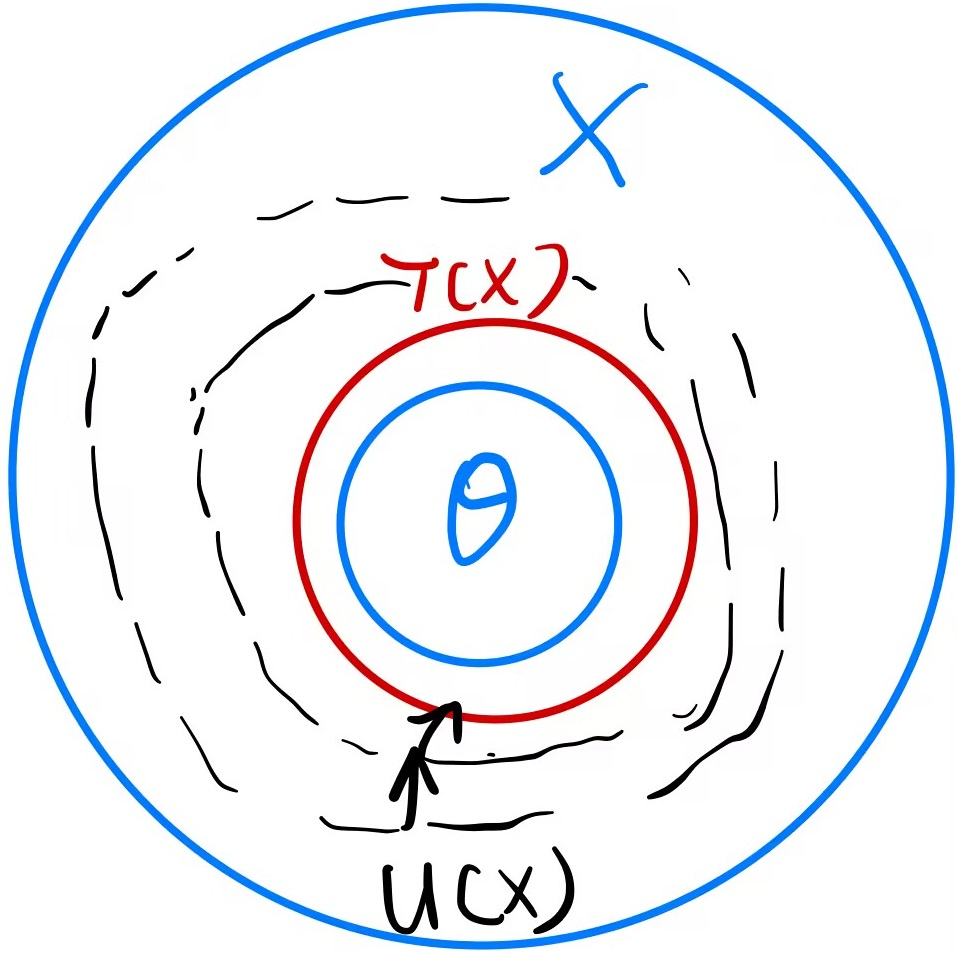
\includegraphics[width=0.41\textwidth]{./figures/chapter1/minimum_sufficient_statistic.png}
\end{figure}
\end{definition}

\begin{proposition}
$T(X),U(X)$ are the sufficient statistic, so
\begin{align*}
I(\theta;T(X)) &= I(\theta;X) \\
I(\theta;U(X)) &= I(\theta;X)
\end{align*}
$T(X)$ is the minimal sufficient statistic, so from data processing inequality:
$$I(X;T(X))\leq I(X;U(X))$$
understanding: 从上面的关系图来看, $T(X)$是对$U(X)$进行不断提纯,仅可能的去掉和$X$相关的信息, 只保留和$\theta$相关的信息.

e.g. 图像分类, 最理想的情况下, $(X,Y)$ 的最小充分统计量是$T(X)=Y$.
\end{proposition}
\chapter{Asymptotic Equipartition Property}

Book Chapter3. (P83)

Asymptotic Equipartition Property(AEP): 等分渐进性. 可以看作大数定理在信息论中的体现.

\section{Law of Large Numbers}

几种收敛方式:
Given a sequence $X_1,X_2,\ldots,X_n$, it converges to $X$:
\begin{itemize}
\item[1.] In probability(依概率收敛):
$$\lim\limits_{n\to\infty}P\left(|X_n-X|>\epsilon\right)=0\Rightarrow\lim\limits_{n\to\infty}P\left(|X_n-X|>\epsilon\right)<\delta$$
\item[2.] In mean square(均方收敛): $\lim\limits_{n\to\infty}\mathbb{E}\left[(X_n-X)^2\right]=0$.
\item[3.] Almost surely / with probability 1: $P\left(\lim\limits_{n\to\infty}X_n=X\right)=1$.
\end{itemize}

Law of Large Numbers(LLN): 大数定律.
$x_1,\ldots,x_n\stackrel{i.i.d.}{\sim}p(x)$, then $\dfrac{1}{n}\sum\limits_{i=1}^nx_i$ converges to $\mathbb{E}[x]$.

(1) in probability: Weak LLN(Weak Law of Large Numbers).

(2) w.p. $1$: Strong LLN(Strong Law of Large Numbers).
\section{Entropy Rates of Stochastic Processes}


\begin{definition}
The \textbf{entropy rate} of a stochastic process $\{X_i\}$ is defined as
$$H\left(\mathcal{X}\right) = \lim_{n\to\infty} \frac{1}{n}H(X_1,X_2,\cdots,X_n)$$
\end{definition}
随机过程$X(t)$的不确定度为$H(X(t))$, 整个随机过程的不确定度为$H\left(\mathcal{X}\right)$. $H\left(\mathcal{X}\right)$平衡整个过程中每个变量的不确定度(信息量), 极限可能不存在(e.g. 趋于极限时$H(\mathcal{X}$)可能在振荡, 而不是收敛到具体值).但$H\left(\mathcal{X}\right)$一定有界:
$$0\leq H(X_i)\leq \log|\mathcal{X}| \Rightarrow 0\leq H\left(\mathcal{X}\right)\leq \log|\mathcal{X}|$$

\begin{example}
\begin{itemize}
\item[1.] $X_1,X_2,\cdots,X_n$ are i.i.d., then:
$$H\left(\mathcal{X}\right) = \lim_{n\to\infty} \dfrac{1}{n}H(X_1,X_2,\cdots,X_n) = \lim_{n\to\infty} \dfrac{1}{n}\sum_{i=1}^nH(X_i) = H(X_1) = \ldots = H(X_n)$$

\item[2.] $X_1\perp X_2\perp\ldots\perp X_n$, then:
$$H\left(\mathcal{X}\right)=\lim_{n\to\infty}\dfrac{1}{n}H(X_1,X_2,\cdots,X_n) = \lim_{n\to\infty}\dfrac{1}{n}\sum_{i=1}^nH(X_i)$$

\end{itemize}
\end{example}

\begin{definition}
Define a related quantity for entropy rate:
$$H'\left(\mathcal{X}\right) = \lim_{n\to\infty}H(X_n|X_{n-1},X_{n-2},\cdots,X_1)$$
\end{definition}

\begin{theorem}
For a stationary stochastic process $\{X(t)\}$, $H\left(\mathcal{X}\right)$ limit exists:
$$H\left(\mathcal{X}\right) = H'\left(\mathcal{X}\right) = \lim_{n\to\infty}H(X_n|X_{n-1},X_{n-2},\cdots,X_1)$$
\end{theorem}

\begin{example}
For a stationary Markov chain: $X_1\rightarrow X_2\rightarrow\cdots\rightarrow X_n$ \textbf{(记忆为1!)}
$$H\left(\mathcal{X}\right)=H'\left(\mathcal{X}\right)=\lim_{n\to\infty}H(X_n|X_{n-1},\ldots,X_1)=H(X_n|X_{n-1})=\ldots=H(X_2|X_1)$$
\end{example}
\section{Fano's Inequality, Channel Coding Theorem(Shannon's Second Theorem)}
简单理解: 从jointly typical set的角度. 在第四章的最后(jointly AEP), 每个$X^n$平均会有$\frac{2^{nH(X,Y)}}{2^{nH(X)}}=2^{nH(Y|X)}$个$Y^n$与之jointly typical, 即将所有的$Y^n$进行划分, 每份的大小为$2^{nH(Y|X)}$, 可以分成 $\frac{2^{nH(Y)}}{2^{nH(Y|X)}}=2^{nI(X;Y)}$份. 这样平均每次用信道发送的bit数为$\frac{2^{nI(X;Y)}}{n}=I(X;Y)$

在保证无损传输的情况下, 信道容量:
$$C\triangleq\max R=\max\limits_{p(x)}I(X;Y)$$

\begin{definition}
Channel Coding Theorem(Shannon's Second Theorem) \\
对于一个rate 为 $R$ 的DMC, 只要$R<C$, 那么这个DMC是 \textcolor{blue}{achievable} 的. i.e. $\forall R<C, \exists$ a sequence of $\left(2^{nR},n\right)$ codes, 使得最大错误概率$\lambda^{(n)}\to 0$. \\
\textcolor{blue}{Conversely}, 任意sequence of $\left(2^{nR},n\right)$ codes, $\lambda^{(n)}\to 0$, 那么$R\leq C$.
\end{definition}
所以证明需要从两个角度: \\
1. 可达性证明(\textcolor{blue}{achievable} proof): $\forall R<C$, $\exists (R,n)$, s.t. $\lambda^{(n)}\to 0$, 找到一种达到$C$的方法. \\
2. \textcolor{blue}{converse} proof: 所有方法都不可能超过$C$. i.e. $R>C$时, $p_e^{(n)}\to 1 \Rightarrow R\leq C$时, $p_e^{(n)}\not\to 0$.


\textcolor{blue}{1. 可达性证明 achievable proof}:

<1>. 码本构建(randomly coding): fixed $p(x)$, 产生$2^{nR}$个长度为$n$的codewords: $X^n(1),\ldots,X^n(2^{nR})\stackrel{i.i.d.}{\sim}p(X^n)=\prod\limits_{i=1}^np(x_i)$.
\begin{figure}[htbp]
    \centering
    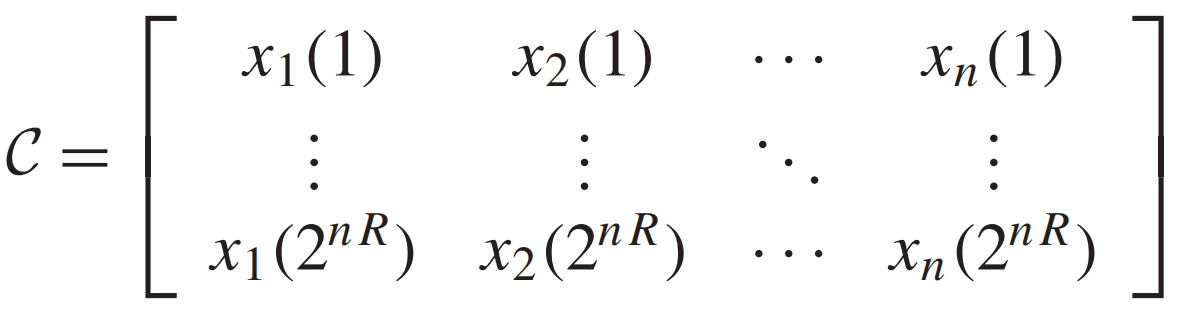
\includegraphics[width=0.5\textwidth]{./figures/chapter5/codebook.png}
\end{figure}

$X_i(w)$表示第$w$个codeword的第$i$个bit(下标为$i$). \\
码本构建好之后发给发送端和接收端(is known by the encoder and the decoder). 同时, 认为sender和receiver知道channel transition matrix $p(y|x)$.

<2>. Encoder: 随机生成一个数字 $w$, $p(W=w)=\dfrac{1}{2^{nR}}$, 从codebook $\mathcal{C}$中找出第$w$行$X^n(w)$, 发到信道当中.

<3> Decoder: reciver 接收由 $p(y^n|x^n(w))=\prod\limits_{i=1}^np(y_i|x_i(w))$ 生成的 $y^n$, 从codebook中找出一条message $\hat{W}$, s.t. $(X^n(\hat{W}), y^n)\in A_{\epsilon}^{(n)}(P_{X,Y})$, 且 no other index $W'\neq \hat{W}$ s.t. $(X^n(W'), y^n)\in A_{\epsilon}^{(n)}(P_{X,Y})$.

若找不到$\hat{W}$, an error is decleared.

<4> Error probability analysis: \\
先忽略码本的随机性 ($p(\mathcal{C})=\prod\limits_{w}^{2^{nR}}\prod\limits_{i=1}^np(x_i)(w)$), 考虑单一码本的情况. \\
发生错误: $\mathcal{E}=\left\{\hat{W}(Y^n) \neq W\right\}$. \\
考虑定义: $\lambda(i)=\Pr\left[\hat{W}\neq i|W=i\right]$, 则 $\Pr\left[\mathcal{E}|W=i\right]=\lambda(i)$. \\
$\Rightarrow \Pr\left[\hat{W}\neq W\right]=\sum\limits_{w=1}^{2^{nR}}p(W=w)\lambda(w)=\sum\limits_{w=1}^{2^{nR}}\dfrac{1}{2^{nR}}\lambda(w)$.

由于$W=1,\ldots,2^{nR}$是等概率产生的, 且地位相同, 所以 W.L.O.G. 取 $W=1$时的情况进行分析:

定义事件 $E_i=\left\{\left(X^{n}(i),Y^n\right)\in A_{\epsilon}^{(n)}(P_{X,Y})\right\}$, i.e. the i-th codeword is joint typical with the received sequence $Y^n$. \\
由jointly AEP, we can get that for sufficiently large $n$:
$$\Pr\left[E_1^c:\left(X^{n}(i),Y^n\right)\not\in A_{\epsilon}^{(n)}(P_{X,Y}) \right]\to 0 \Rightarrow \Pr\left[E_1^c: \left(X^{n}(i),Y^n\right)\not\in A_{\epsilon}^{(n)}(P_{X,Y})\right]\leq \epsilon$$
由于生成codebook $\mathcal{C}$时, 每一行的产生是独立的, i.e. $X^n(1)$与$X^n(2),\ldots,X^n(2^{nR})$是独立的, 所以$Y^n$与$X^n(i)$也是独立的, 所以有:
$$\Pr\left[E_i:\left(X^{n}(i),Y^n\right)\in A_{\epsilon}^{(n)}(P_{X,Y}) \right]\leq 2^{-n\left(I(X;Y)-3\epsilon\right)}$$
由jointly AEP, 当$R<I(X;Y)-3\epsilon$时
\begin{align*}
\Pr\left[\hat{W}\neq 1|W=1\right] &= \Pr\left[E_1^c\cup E_2\cup\ldots\cup E_{2^{nR}}\right] \\
&\leq \Pr\left[E_1^c\right] + \sum\limits_{w=2}^{2^{nR}}\Pr\left[E_w\right] \\
&\leq \epsilon + (2^{nR}-1) 2^{-n\left(I(X;Y)-3\epsilon\right)} \\
&\leq \epsilon + 2^{n\left(R-I(X;Y)+3\epsilon\right)} \\
&\leq 2\epsilon \quad \text{(sufficiently large $n$, $R<I(X;Y)-3\epsilon\Rightarrow 2^{n\left(R-I(X;Y)+3\epsilon\right)}\to 0<\epsilon$)}
\end{align*}
总结: 选择证明中取等时的分布作为真实分布 $p(x)\gets p^*(x)$, 此时$\forall R<I(X;Y)-3\epsilon$, i.e. $R<C$, 错误概率$p_e^{(n)}=\Pr\left[\hat{W}\neq W\right]\to 0\Rightarrow \lambda^{(n)}\to 0$. (Actually, $\lambda^{(n)}$条件比$p_e^{(n)}$更强, 但是$p_e^{(n)}$更容易计算)

若将codebook $\mathcal{C}$ 的随机性也考虑进去, 则会得到更加平均的结果:
$$\Pr\left[\hat{W}\neq W\right]=\sum_{w=1}^{2^{nR}}\sum_{\mathcal{C}}\Pr[\mathcal{C}]\dfrac{1}{2^{nR}}\lambda_w(\mathcal{C})=\lambda_1(\mathcal{C})\Rightarrow \Pr(\mathcal{E}|\mathcal{C}^*)\leq 2\epsilon$$
The best codebook $\mathcal{C}^*$ 中必然由超过一半的indices $i$ and their assciated codewords $X^n(i)$, 满足 $\lambda_i\leq 4\epsilon$, 否则$\Pr(\mathcal{E}|\mathcal{C}^*)>2\epsilon$. 砍去另一半codewords, 可以得到rate为$R'=\dfrac{\frac{2^{nR}}{2}}{n}=R-\dfrac{1}{n}$, s.t. $\lambda^{(n)}\leq 4\epsilon\to 0$. 所以可以使得 $\epsilon$ 不断的取小, 说明了$R$可以取到$C$的任意接近的地方.(取$p^*(x)$时, $C=I(X;Y), R=I(X;Y)-3\epsilon\to C$)

由此证明了 Achievability.

\begin{proposition}
Zero-error codes.
$$p_e^{(n)}\to 0 \Rightarrow R\leq C$$
\end{proposition}
proof: \\
Channel encoding 满足Markov chain $W\to X^n(W)\to Y^n\to \hat{W}$, so from data-processing inequality:
$$I(W; Y^n)\leq I(X^n(W); Y^n)$$

由 DMC的 memoryless, i.e. $p(Y_i|Y_1,\ldots,Y_{i-1},X^n)=p(Y_i|X_i)$, so
\begin{align*}
I(X^n;Y^n) &= H(Y^n) - H(Y^n|X^n) \\
&= \sum_{i=1}^nH(Y_i|Y_1,\ldots,Y_{i-1}) - \sum_{i=1}^nH(Y_i|Y_1,\ldots,Y_{i-1}, X^n) \\
&\leq \sum_{i=1}^nH(Y_i) - \sum_{i=1}^nH(Y_i|X_i) \qquad \text{(memoryless \& conditioning reduced entropy)} \\
&= \sum_{i=1}^n I(X_i;Y_i) \\
&\leq nC \qquad\qquad\qquad\qquad\qquad\quad\ \ \text{($Y_i$ are independent, $p_i(x)=p^*(x)$)}
\end{align*}

Since the channel is zero-error, so $\hat{W}=g(Y^n)=W$, i.e. $H(W|Y^n)=0$.
\begin{align*}
nR &= H(W) \\
&= H(W|Y^n) + I(W;Y^n) \\
&= I(W;Y^n) \qquad\quad\ \text{($H(W|Y^n)=0$)} \\
&\leq I(X^n;Y^n) \qquad\quad \text{(data-processing inequality)} \\
&\leq nC
\end{align*}

So for any zero-error $\left(2^{nR}, n\right)$ code, for all $n$:
$$R\leq C$$

\textcolor{blue}{2. converse proof: 证明$R>C$时, $p_e^{(n)}\to 1$ or $p_e^{(n)}\not\to 0$ as $n\to\infty$.}

\begin{definition}
Fano's Inequality: 是关于$p_e$的函数, 建立条件熵和错误概率$p_e$的关系. \\
For any estimator $\hat{X}$ such that $X\to Y\to \hat{X}$, $p_e=P(\hat{X}\neq X)$, then
$$H(p_e)+p_e\log\left|\mathcal{X}\right|\geq H(X|\hat{X})\geq H(X|Y)$$
It could be weakened to:
$$1+p_e\log\left|\mathcal{X}\right|\geq H(X|\hat{X})\geq H(X|Y)$$
or
$$p_e\geq \frac{H(X|Y)-1}{\log\left|\mathcal{X}\right|}$$
\end{definition}

Proof: \\
Let $E$ be the auxiliary variable indicate where the prediction is correct. i.e.
$$E=\begin{cases}
    1, & \text{if } \hat{X}\neq X \\
    0, & \text{if } \hat{X}=X
\end{cases}$$
Then we have $p(E=1)=p_e$, so
\begin{align*}
H\left(E,X|\hat{X}\right) &= \underbrace{H\left(E|\hat{X}\right)}_{\leq H(p_e)}+\underbrace{H\left(X|E,\hat{X}\right)}_{\leq p_e\log\left|\mathcal{X}\right|} \\
&= H\left(X|\hat{X}\right)+\underbrace{H\left(E|X,\hat{X}\right)}_{=0}
\end{align*}
其中由于$E=\mathbb{I}_{X=\hat{X}}$, 所以$H\left(E|X,\hat{X}\right)=0$. \\
由于conditioning reduces entropy, 所以 $H\left(E|\hat{X}\right)\leq H(E)=H(p_e)$. \\
同时有当$E=1$时, 给定$\hat{X}$, $X$的取值共有$\left|\mathcal{X}\right|-1$种, 所以有:
\begin{align*}
H\left(X|E, \hat{X}\right) &= \sum_{e=0,1}H\left(X|E=e, \hat{X}\right)P(E=e) \\
&\leq p_e\log\left(\left|\mathcal{X}\right|-1\right) + (1-p_e)\cdot 0 \\
&\leq p_e\log\left|\mathcal{X}\right|
\end{align*}
综上, 可以得到 Fano's Inequality:
$$H(p_e)+p_e\log\left|\mathcal{X}\right|\geq H(X|\hat{X})$$
weakened to的版本可由$H\left(p_e\right)\leq 1$, 以及数据处理不等式得到:
$$I(X;Y)\geq I(X;\hat{X})\Rightarrow H(X)-H(X|Y)\geq H(X)-H(X|\hat{X})\Rightarrow H(X|\hat{X})\geq H(X|Y)$$

由于 Channel encoding 满足Markov chain $W\to X^n(W)\to Y^n\to \hat{W}$, 所以应用Fano's Inequality:
$$H(W|\hat{W})\leq H(p_e^{(n)})+p_e^{(n)}\log\left|\mathcal{W}\right|$$
其中$\mathcal{W}=\left\{1,\ldots,2^{nR}\right\}$, 所以 $\left|\mathcal{W}\right|=2^{nR}\Rightarrow \log\left|\mathcal{W}\right|=nR$, 由于$W$是等概率产生的, 所以$H(W)= \log\left|\mathcal{W}\right| = nR$. 所以有
\begin{align*}
nR &= H(W) \\
&= H(W|\hat{W}) + I(W;\hat{W}) \qquad\qquad\quad \text{(definition of mutual information)} \\
&\leq H(p_e^{(n)})+p_e^{(n)} nR + I(W;\hat{W}) \qquad \text{(Fano's Inequality)} \\
&\leq 1 + p_e^{(n)}nR + nC \qquad \text{($I(W;\hat{W})\leq I(X^n;Y^n)\leq nC$ proved in zero-error code part)} \\
\Rightarrow R &\leq \dfrac{1}{n} + p_e^{(n)}R + C \\
\Rightarrow p_e^{(n)} &\geq 1 - \dfrac{C}{R} - \dfrac{1}{nR}
\end{align*}

取等条件: $W,\hat{W}$ 无信息丢失(zero-error code), i.e. $X^n=f(W), Y^n=g(X^n)$是$W$的充分统计量, $W$到$\hat{W}$是一对一的映射. 由充分统计量(s.s.), 此时可以看作构成 Markov Chain:
\begin{align*}
W \to X^n \to Y^n \to \hat{W} \\
W \to \hat{W} \to X^n \to Y^n
\end{align*}

由于我们的前提假设是 $R>C$, 且 $R,C$ 为常数, 所以 $\dfrac{C}{R}<1$, 是常数. 当$n\to\infty$时, $\dfrac{1}{nR}\to 0<\epsilon$, 所以 $p_e^{(n)}\geq 1-\text{(constant less than $1$)} - \epsilon \not\to 0$.

所以我们证明了 $\forall R>C, p_e^{(n)}\not\to 0$, 即证明了converse proof.
\section{Sufficient Statistics}
Background: $X_1,\cdots,X_n\sim \left\{f_{\theta}(X)\right\}=\left\{\mathcal{N}(\theta,1)\right\}$(a family of distribution, 一族元素), try to estimate the unknown parameter $\theta$s with the samples $X_1,\cdots,X_n$.

用MLE估计$\theta$时, 我们知道:
$$\hat{\theta} = \dfrac{\sum\limits_{i=1}^n X_i}{n}$$
所以拥有全部样本$X_1,\cdots,X_n$, 以及$T(X_1,\cdots,X_n)=\dfrac{\sum\limits_{i=1}^n X_i}{n}$, 对于预测$\theta$的效果是相同的$\Rightarrow$ 大大减少了数据储存量.

两者对参数的估计效果相同: $T(X_1,\cdots,X_n)$对变量的操作没有信息损失!

\begin{definition}
$T(X_1,\cdots,X_n)$ is the sufficient statistic(s.s.), if the Markov chain holds:
$$\theta\leftrightarrow T\left(X_1,\cdots,X_n\right)\leftrightarrow \left(X_1,\cdots,X_n\right)$$
\end{definition}
由于$X\leftrightarrow Y\leftrightarrow g(Y)$天然成立, 所以$$\theta\leftrightarrow \left(X_1,\cdots,X_n\right) \leftrightarrow T\left(X_1,\cdots,X_n\right)$$
From the data processing Inequality, we have:
\begin{align*}
I\left(\theta;T\left(X_1,\cdots,X_n\right)\right) &\geq I\left(\theta;\left(X_1,\cdots,X_n\right)\right) \\
I\left(\theta;\left(X_1,\cdots,X_n\right)\right) &\geq I\left(\theta;T\left(X_1,\cdots,X_n\right)\right) \\
\textcolor{red}{I\left(\theta;\left(X_1,\cdots,X_n\right)\right)} &\textcolor{red}{= I\left(\theta;T\left(X_1,\cdots,X_n\right)\right)}
\end{align*}

\begin{example}
$X_1,\cdots,X_n \stackrel{i.i.d.}{\sim} Bern(\theta)$, $n$ is known.
The sufficient statistic is
$$T(X_1,\cdots,X_n)=\sum_{i=1}^n X_i$$
prove:
$$P\left[(X_1,\cdots,X_n)=(x_1,\cdots,x_n)\big|\sum_{i=1}^nX_i=k\right]=\dfrac{1}{\binom{n}{k}}$$
与$\theta$无关, 所以$T(X_1,\cdots,X_n)$是充分统计量.
\end{example}

\begin{example}
$X_1,\cdots,X_n \stackrel{i.i.d.}{\sim} \mathcal{N}(\mu,\sigma^2)$.
$$\mu\leftrightarrow \text{样本均值} \leftrightarrow \left(X_1,\cdots,X_n\right)$$
$$\sigma\leftrightarrow \text{样本方差} \leftrightarrow \left(X_1,\cdots,X_n\right)$$
\end{example}

\begin{example}
$f_{\theta}=Unif(\theta,\theta+1)$\\
$T(X_1,\cdots,X_n)=\left\{\min\left\{X_1,\cdots,X_n\right\},\max\left\{X_1,\cdots,X_n\right\}\right\}$

simply prove:
Since $X_1, \ldots, X_n\stackrel{i.i.d}{\sim}\operatorname{Unif}(\theta, \theta+1)$, so the PDF:
$$f\left(x_i \mid \theta\right)= \mathbb{I}_{\theta\leq x_i \leq \theta+1}$$
The joint distribution is:
$$f\left(x_1, \ldots, x_n \mid \theta\right) = \prod_{i=1}^n f\left(x_i \mid \theta\right) = \mathbb{I}_{\theta \leq \min \left\{x_1, \ldots, x_n\right\} \& \max \left\{x_1, \ldots, x_n\right\} \leq \theta+1}$$
when $\theta \leq \min \left\{x_1, \ldots, x_n\right\}, \left\{x_1, \ldots, x_n\right\} \leq \theta+1$, $g\left(T\left(x_1, \ldots, x_n\right), \theta\right)=1$. \\
So $T(X)=\left\{\min \left\{X_1, \ldots, X_n\right\}, \max \left\{X_1, \ldots, X_n\right\}\right\}$ is a sufficient statistic.

\end{example}

\begin{proposition}
充分统计量可能不唯一. e.g. $\forall k$
\begin{align*}
\theta &\leftrightarrow X \leftrightarrow X+k \\
\theta &\leftrightarrow X+k \leftrightarrow X
\end{align*}
\end{proposition}

\begin{definition}
所以引入最小充分统计量(minimal sufficient statistic):
$T(X)$ is the minimal sufficient statistic, if for any other sufficient statistic $U(X)$ has:
$$\theta\leftrightarrow T(X)\leftrightarrow U(X)\leftrightarrow X$$
\begin{figure}[htbp]
    \centering
    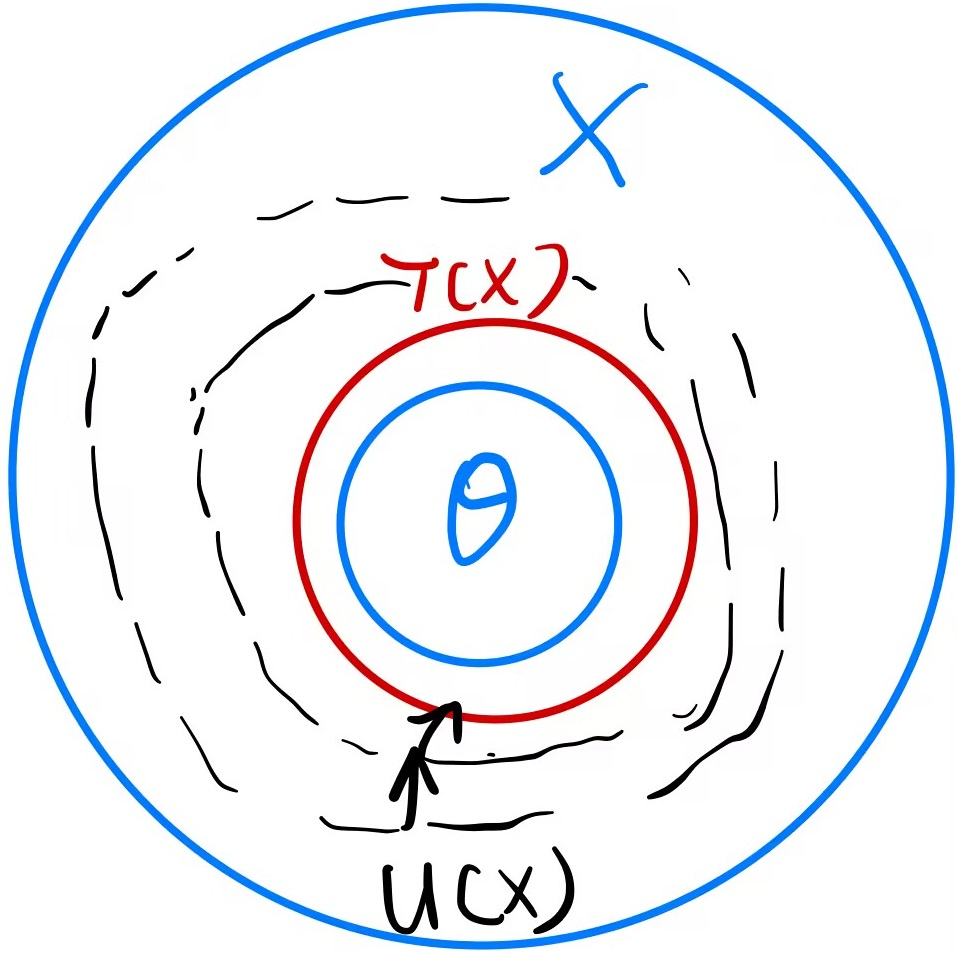
\includegraphics[width=0.41\textwidth]{./figures/chapter1/minimum_sufficient_statistic.png}
\end{figure}
\end{definition}

\begin{proposition}
$T(X),U(X)$ are the sufficient statistic, so
\begin{align*}
I(\theta;T(X)) &= I(\theta;X) \\
I(\theta;U(X)) &= I(\theta;X)
\end{align*}
$T(X)$ is the minimal sufficient statistic, so from data processing inequality:
$$I(X;T(X))\leq I(X;U(X))$$
understanding: 从上面的关系图来看, $T(X)$是对$U(X)$进行不断提纯,仅可能的去掉和$X$相关的信息, 只保留和$\theta$相关的信息.

e.g. 图像分类, 最理想的情况下, $(X,Y)$ 的最小充分统计量是$T(X)=Y$.
\end{proposition}
\section{Other codes*}
\begin{itemize}
\item Reed-Muller Code: 利用$\mathcal{C}$的线性性质.
\item Hudmard Code: 参数选择上有限制($n=2^m$)
\item LDPC Code(Low-Density Parity-Check Code) :5G中常用的编码方式, 逼近Shannon channel capacity
\end{itemize}
Details in PPT Lecture 4 Channle Encoding.
\chapter{Channel Capacity}

信道容量. \qquad Book Chapter7. (P209)

Source Encoding(信源编码): 为了减少信源冗余度而进行的信源符号变换. 针对信源输出符号序列的统计特性, 把信源输出符号序列变换为最短的码字序列. 目的是数据压缩, 模数转换.

Channel Encoding(信道编码): 为了对抗信道中的噪音和衰减, 通过增加冗余来提高抗干扰能力和纠错能力, 提高信道传输可靠性.

\section{Law of Large Numbers}

几种收敛方式:
Given a sequence $X_1,X_2,\ldots,X_n$, it converges to $X$:
\begin{itemize}
\item[1.] In probability(依概率收敛):
$$\lim\limits_{n\to\infty}P\left(|X_n-X|>\epsilon\right)=0\Rightarrow\lim\limits_{n\to\infty}P\left(|X_n-X|>\epsilon\right)<\delta$$
\item[2.] In mean square(均方收敛): $\lim\limits_{n\to\infty}\mathbb{E}\left[(X_n-X)^2\right]=0$.
\item[3.] Almost surely / with probability 1: $P\left(\lim\limits_{n\to\infty}X_n=X\right)=1$.
\end{itemize}

Law of Large Numbers(LLN): 大数定律.
$x_1,\ldots,x_n\stackrel{i.i.d.}{\sim}p(x)$, then $\dfrac{1}{n}\sum\limits_{i=1}^nx_i$ converges to $\mathbb{E}[x]$.

(1) in probability: Weak LLN(Weak Law of Large Numbers).

(2) w.p. $1$: Strong LLN(Strong Law of Large Numbers).
\section{Entropy Rates of Stochastic Processes}


\begin{definition}
The \textbf{entropy rate} of a stochastic process $\{X_i\}$ is defined as
$$H\left(\mathcal{X}\right) = \lim_{n\to\infty} \frac{1}{n}H(X_1,X_2,\cdots,X_n)$$
\end{definition}
随机过程$X(t)$的不确定度为$H(X(t))$, 整个随机过程的不确定度为$H\left(\mathcal{X}\right)$. $H\left(\mathcal{X}\right)$平衡整个过程中每个变量的不确定度(信息量), 极限可能不存在(e.g. 趋于极限时$H(\mathcal{X}$)可能在振荡, 而不是收敛到具体值).但$H\left(\mathcal{X}\right)$一定有界:
$$0\leq H(X_i)\leq \log|\mathcal{X}| \Rightarrow 0\leq H\left(\mathcal{X}\right)\leq \log|\mathcal{X}|$$

\begin{example}
\begin{itemize}
\item[1.] $X_1,X_2,\cdots,X_n$ are i.i.d., then:
$$H\left(\mathcal{X}\right) = \lim_{n\to\infty} \dfrac{1}{n}H(X_1,X_2,\cdots,X_n) = \lim_{n\to\infty} \dfrac{1}{n}\sum_{i=1}^nH(X_i) = H(X_1) = \ldots = H(X_n)$$

\item[2.] $X_1\perp X_2\perp\ldots\perp X_n$, then:
$$H\left(\mathcal{X}\right)=\lim_{n\to\infty}\dfrac{1}{n}H(X_1,X_2,\cdots,X_n) = \lim_{n\to\infty}\dfrac{1}{n}\sum_{i=1}^nH(X_i)$$

\end{itemize}
\end{example}

\begin{definition}
Define a related quantity for entropy rate:
$$H'\left(\mathcal{X}\right) = \lim_{n\to\infty}H(X_n|X_{n-1},X_{n-2},\cdots,X_1)$$
\end{definition}

\begin{theorem}
For a stationary stochastic process $\{X(t)\}$, $H\left(\mathcal{X}\right)$ limit exists:
$$H\left(\mathcal{X}\right) = H'\left(\mathcal{X}\right) = \lim_{n\to\infty}H(X_n|X_{n-1},X_{n-2},\cdots,X_1)$$
\end{theorem}

\begin{example}
For a stationary Markov chain: $X_1\rightarrow X_2\rightarrow\cdots\rightarrow X_n$ \textbf{(记忆为1!)}
$$H\left(\mathcal{X}\right)=H'\left(\mathcal{X}\right)=\lim_{n\to\infty}H(X_n|X_{n-1},\ldots,X_1)=H(X_n|X_{n-1})=\ldots=H(X_2|X_1)$$
\end{example}
\section{Fano's Inequality, Channel Coding Theorem(Shannon's Second Theorem)}
简单理解: 从jointly typical set的角度. 在第四章的最后(jointly AEP), 每个$X^n$平均会有$\frac{2^{nH(X,Y)}}{2^{nH(X)}}=2^{nH(Y|X)}$个$Y^n$与之jointly typical, 即将所有的$Y^n$进行划分, 每份的大小为$2^{nH(Y|X)}$, 可以分成 $\frac{2^{nH(Y)}}{2^{nH(Y|X)}}=2^{nI(X;Y)}$份. 这样平均每次用信道发送的bit数为$\frac{2^{nI(X;Y)}}{n}=I(X;Y)$

在保证无损传输的情况下, 信道容量:
$$C\triangleq\max R=\max\limits_{p(x)}I(X;Y)$$

\begin{definition}
Channel Coding Theorem(Shannon's Second Theorem) \\
对于一个rate 为 $R$ 的DMC, 只要$R<C$, 那么这个DMC是 \textcolor{blue}{achievable} 的. i.e. $\forall R<C, \exists$ a sequence of $\left(2^{nR},n\right)$ codes, 使得最大错误概率$\lambda^{(n)}\to 0$. \\
\textcolor{blue}{Conversely}, 任意sequence of $\left(2^{nR},n\right)$ codes, $\lambda^{(n)}\to 0$, 那么$R\leq C$.
\end{definition}
所以证明需要从两个角度: \\
1. 可达性证明(\textcolor{blue}{achievable} proof): $\forall R<C$, $\exists (R,n)$, s.t. $\lambda^{(n)}\to 0$, 找到一种达到$C$的方法. \\
2. \textcolor{blue}{converse} proof: 所有方法都不可能超过$C$. i.e. $R>C$时, $p_e^{(n)}\to 1 \Rightarrow R\leq C$时, $p_e^{(n)}\not\to 0$.


\textcolor{blue}{1. 可达性证明 achievable proof}:

<1>. 码本构建(randomly coding): fixed $p(x)$, 产生$2^{nR}$个长度为$n$的codewords: $X^n(1),\ldots,X^n(2^{nR})\stackrel{i.i.d.}{\sim}p(X^n)=\prod\limits_{i=1}^np(x_i)$.
\begin{figure}[htbp]
    \centering
    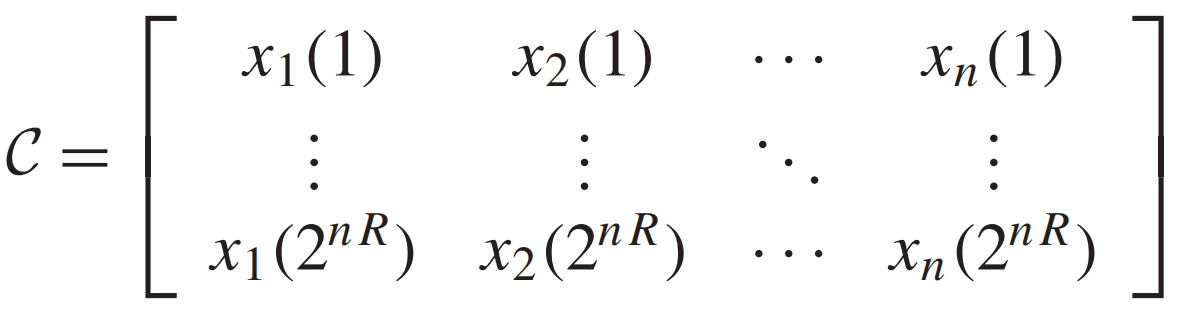
\includegraphics[width=0.5\textwidth]{./figures/chapter5/codebook.png}
\end{figure}

$X_i(w)$表示第$w$个codeword的第$i$个bit(下标为$i$). \\
码本构建好之后发给发送端和接收端(is known by the encoder and the decoder). 同时, 认为sender和receiver知道channel transition matrix $p(y|x)$.

<2>. Encoder: 随机生成一个数字 $w$, $p(W=w)=\dfrac{1}{2^{nR}}$, 从codebook $\mathcal{C}$中找出第$w$行$X^n(w)$, 发到信道当中.

<3> Decoder: reciver 接收由 $p(y^n|x^n(w))=\prod\limits_{i=1}^np(y_i|x_i(w))$ 生成的 $y^n$, 从codebook中找出一条message $\hat{W}$, s.t. $(X^n(\hat{W}), y^n)\in A_{\epsilon}^{(n)}(P_{X,Y})$, 且 no other index $W'\neq \hat{W}$ s.t. $(X^n(W'), y^n)\in A_{\epsilon}^{(n)}(P_{X,Y})$.

若找不到$\hat{W}$, an error is decleared.

<4> Error probability analysis: \\
先忽略码本的随机性 ($p(\mathcal{C})=\prod\limits_{w}^{2^{nR}}\prod\limits_{i=1}^np(x_i)(w)$), 考虑单一码本的情况. \\
发生错误: $\mathcal{E}=\left\{\hat{W}(Y^n) \neq W\right\}$. \\
考虑定义: $\lambda(i)=\Pr\left[\hat{W}\neq i|W=i\right]$, 则 $\Pr\left[\mathcal{E}|W=i\right]=\lambda(i)$. \\
$\Rightarrow \Pr\left[\hat{W}\neq W\right]=\sum\limits_{w=1}^{2^{nR}}p(W=w)\lambda(w)=\sum\limits_{w=1}^{2^{nR}}\dfrac{1}{2^{nR}}\lambda(w)$.

由于$W=1,\ldots,2^{nR}$是等概率产生的, 且地位相同, 所以 W.L.O.G. 取 $W=1$时的情况进行分析:

定义事件 $E_i=\left\{\left(X^{n}(i),Y^n\right)\in A_{\epsilon}^{(n)}(P_{X,Y})\right\}$, i.e. the i-th codeword is joint typical with the received sequence $Y^n$. \\
由jointly AEP, we can get that for sufficiently large $n$:
$$\Pr\left[E_1^c:\left(X^{n}(i),Y^n\right)\not\in A_{\epsilon}^{(n)}(P_{X,Y}) \right]\to 0 \Rightarrow \Pr\left[E_1^c: \left(X^{n}(i),Y^n\right)\not\in A_{\epsilon}^{(n)}(P_{X,Y})\right]\leq \epsilon$$
由于生成codebook $\mathcal{C}$时, 每一行的产生是独立的, i.e. $X^n(1)$与$X^n(2),\ldots,X^n(2^{nR})$是独立的, 所以$Y^n$与$X^n(i)$也是独立的, 所以有:
$$\Pr\left[E_i:\left(X^{n}(i),Y^n\right)\in A_{\epsilon}^{(n)}(P_{X,Y}) \right]\leq 2^{-n\left(I(X;Y)-3\epsilon\right)}$$
由jointly AEP, 当$R<I(X;Y)-3\epsilon$时
\begin{align*}
\Pr\left[\hat{W}\neq 1|W=1\right] &= \Pr\left[E_1^c\cup E_2\cup\ldots\cup E_{2^{nR}}\right] \\
&\leq \Pr\left[E_1^c\right] + \sum\limits_{w=2}^{2^{nR}}\Pr\left[E_w\right] \\
&\leq \epsilon + (2^{nR}-1) 2^{-n\left(I(X;Y)-3\epsilon\right)} \\
&\leq \epsilon + 2^{n\left(R-I(X;Y)+3\epsilon\right)} \\
&\leq 2\epsilon \quad \text{(sufficiently large $n$, $R<I(X;Y)-3\epsilon\Rightarrow 2^{n\left(R-I(X;Y)+3\epsilon\right)}\to 0<\epsilon$)}
\end{align*}
总结: 选择证明中取等时的分布作为真实分布 $p(x)\gets p^*(x)$, 此时$\forall R<I(X;Y)-3\epsilon$, i.e. $R<C$, 错误概率$p_e^{(n)}=\Pr\left[\hat{W}\neq W\right]\to 0\Rightarrow \lambda^{(n)}\to 0$. (Actually, $\lambda^{(n)}$条件比$p_e^{(n)}$更强, 但是$p_e^{(n)}$更容易计算)

若将codebook $\mathcal{C}$ 的随机性也考虑进去, 则会得到更加平均的结果:
$$\Pr\left[\hat{W}\neq W\right]=\sum_{w=1}^{2^{nR}}\sum_{\mathcal{C}}\Pr[\mathcal{C}]\dfrac{1}{2^{nR}}\lambda_w(\mathcal{C})=\lambda_1(\mathcal{C})\Rightarrow \Pr(\mathcal{E}|\mathcal{C}^*)\leq 2\epsilon$$
The best codebook $\mathcal{C}^*$ 中必然由超过一半的indices $i$ and their assciated codewords $X^n(i)$, 满足 $\lambda_i\leq 4\epsilon$, 否则$\Pr(\mathcal{E}|\mathcal{C}^*)>2\epsilon$. 砍去另一半codewords, 可以得到rate为$R'=\dfrac{\frac{2^{nR}}{2}}{n}=R-\dfrac{1}{n}$, s.t. $\lambda^{(n)}\leq 4\epsilon\to 0$. 所以可以使得 $\epsilon$ 不断的取小, 说明了$R$可以取到$C$的任意接近的地方.(取$p^*(x)$时, $C=I(X;Y), R=I(X;Y)-3\epsilon\to C$)

由此证明了 Achievability.

\begin{proposition}
Zero-error codes.
$$p_e^{(n)}\to 0 \Rightarrow R\leq C$$
\end{proposition}
proof: \\
Channel encoding 满足Markov chain $W\to X^n(W)\to Y^n\to \hat{W}$, so from data-processing inequality:
$$I(W; Y^n)\leq I(X^n(W); Y^n)$$

由 DMC的 memoryless, i.e. $p(Y_i|Y_1,\ldots,Y_{i-1},X^n)=p(Y_i|X_i)$, so
\begin{align*}
I(X^n;Y^n) &= H(Y^n) - H(Y^n|X^n) \\
&= \sum_{i=1}^nH(Y_i|Y_1,\ldots,Y_{i-1}) - \sum_{i=1}^nH(Y_i|Y_1,\ldots,Y_{i-1}, X^n) \\
&\leq \sum_{i=1}^nH(Y_i) - \sum_{i=1}^nH(Y_i|X_i) \qquad \text{(memoryless \& conditioning reduced entropy)} \\
&= \sum_{i=1}^n I(X_i;Y_i) \\
&\leq nC \qquad\qquad\qquad\qquad\qquad\quad\ \ \text{($Y_i$ are independent, $p_i(x)=p^*(x)$)}
\end{align*}

Since the channel is zero-error, so $\hat{W}=g(Y^n)=W$, i.e. $H(W|Y^n)=0$.
\begin{align*}
nR &= H(W) \\
&= H(W|Y^n) + I(W;Y^n) \\
&= I(W;Y^n) \qquad\quad\ \text{($H(W|Y^n)=0$)} \\
&\leq I(X^n;Y^n) \qquad\quad \text{(data-processing inequality)} \\
&\leq nC
\end{align*}

So for any zero-error $\left(2^{nR}, n\right)$ code, for all $n$:
$$R\leq C$$

\textcolor{blue}{2. converse proof: 证明$R>C$时, $p_e^{(n)}\to 1$ or $p_e^{(n)}\not\to 0$ as $n\to\infty$.}

\begin{definition}
Fano's Inequality: 是关于$p_e$的函数, 建立条件熵和错误概率$p_e$的关系. \\
For any estimator $\hat{X}$ such that $X\to Y\to \hat{X}$, $p_e=P(\hat{X}\neq X)$, then
$$H(p_e)+p_e\log\left|\mathcal{X}\right|\geq H(X|\hat{X})\geq H(X|Y)$$
It could be weakened to:
$$1+p_e\log\left|\mathcal{X}\right|\geq H(X|\hat{X})\geq H(X|Y)$$
or
$$p_e\geq \frac{H(X|Y)-1}{\log\left|\mathcal{X}\right|}$$
\end{definition}

Proof: \\
Let $E$ be the auxiliary variable indicate where the prediction is correct. i.e.
$$E=\begin{cases}
    1, & \text{if } \hat{X}\neq X \\
    0, & \text{if } \hat{X}=X
\end{cases}$$
Then we have $p(E=1)=p_e$, so
\begin{align*}
H\left(E,X|\hat{X}\right) &= \underbrace{H\left(E|\hat{X}\right)}_{\leq H(p_e)}+\underbrace{H\left(X|E,\hat{X}\right)}_{\leq p_e\log\left|\mathcal{X}\right|} \\
&= H\left(X|\hat{X}\right)+\underbrace{H\left(E|X,\hat{X}\right)}_{=0}
\end{align*}
其中由于$E=\mathbb{I}_{X=\hat{X}}$, 所以$H\left(E|X,\hat{X}\right)=0$. \\
由于conditioning reduces entropy, 所以 $H\left(E|\hat{X}\right)\leq H(E)=H(p_e)$. \\
同时有当$E=1$时, 给定$\hat{X}$, $X$的取值共有$\left|\mathcal{X}\right|-1$种, 所以有:
\begin{align*}
H\left(X|E, \hat{X}\right) &= \sum_{e=0,1}H\left(X|E=e, \hat{X}\right)P(E=e) \\
&\leq p_e\log\left(\left|\mathcal{X}\right|-1\right) + (1-p_e)\cdot 0 \\
&\leq p_e\log\left|\mathcal{X}\right|
\end{align*}
综上, 可以得到 Fano's Inequality:
$$H(p_e)+p_e\log\left|\mathcal{X}\right|\geq H(X|\hat{X})$$
weakened to的版本可由$H\left(p_e\right)\leq 1$, 以及数据处理不等式得到:
$$I(X;Y)\geq I(X;\hat{X})\Rightarrow H(X)-H(X|Y)\geq H(X)-H(X|\hat{X})\Rightarrow H(X|\hat{X})\geq H(X|Y)$$

由于 Channel encoding 满足Markov chain $W\to X^n(W)\to Y^n\to \hat{W}$, 所以应用Fano's Inequality:
$$H(W|\hat{W})\leq H(p_e^{(n)})+p_e^{(n)}\log\left|\mathcal{W}\right|$$
其中$\mathcal{W}=\left\{1,\ldots,2^{nR}\right\}$, 所以 $\left|\mathcal{W}\right|=2^{nR}\Rightarrow \log\left|\mathcal{W}\right|=nR$, 由于$W$是等概率产生的, 所以$H(W)= \log\left|\mathcal{W}\right| = nR$. 所以有
\begin{align*}
nR &= H(W) \\
&= H(W|\hat{W}) + I(W;\hat{W}) \qquad\qquad\quad \text{(definition of mutual information)} \\
&\leq H(p_e^{(n)})+p_e^{(n)} nR + I(W;\hat{W}) \qquad \text{(Fano's Inequality)} \\
&\leq 1 + p_e^{(n)}nR + nC \qquad \text{($I(W;\hat{W})\leq I(X^n;Y^n)\leq nC$ proved in zero-error code part)} \\
\Rightarrow R &\leq \dfrac{1}{n} + p_e^{(n)}R + C \\
\Rightarrow p_e^{(n)} &\geq 1 - \dfrac{C}{R} - \dfrac{1}{nR}
\end{align*}

取等条件: $W,\hat{W}$ 无信息丢失(zero-error code), i.e. $X^n=f(W), Y^n=g(X^n)$是$W$的充分统计量, $W$到$\hat{W}$是一对一的映射. 由充分统计量(s.s.), 此时可以看作构成 Markov Chain:
\begin{align*}
W \to X^n \to Y^n \to \hat{W} \\
W \to \hat{W} \to X^n \to Y^n
\end{align*}

由于我们的前提假设是 $R>C$, 且 $R,C$ 为常数, 所以 $\dfrac{C}{R}<1$, 是常数. 当$n\to\infty$时, $\dfrac{1}{nR}\to 0<\epsilon$, 所以 $p_e^{(n)}\geq 1-\text{(constant less than $1$)} - \epsilon \not\to 0$.

所以我们证明了 $\forall R>C, p_e^{(n)}\not\to 0$, 即证明了converse proof.
\section{Sufficient Statistics}
Background: $X_1,\cdots,X_n\sim \left\{f_{\theta}(X)\right\}=\left\{\mathcal{N}(\theta,1)\right\}$(a family of distribution, 一族元素), try to estimate the unknown parameter $\theta$s with the samples $X_1,\cdots,X_n$.

用MLE估计$\theta$时, 我们知道:
$$\hat{\theta} = \dfrac{\sum\limits_{i=1}^n X_i}{n}$$
所以拥有全部样本$X_1,\cdots,X_n$, 以及$T(X_1,\cdots,X_n)=\dfrac{\sum\limits_{i=1}^n X_i}{n}$, 对于预测$\theta$的效果是相同的$\Rightarrow$ 大大减少了数据储存量.

两者对参数的估计效果相同: $T(X_1,\cdots,X_n)$对变量的操作没有信息损失!

\begin{definition}
$T(X_1,\cdots,X_n)$ is the sufficient statistic(s.s.), if the Markov chain holds:
$$\theta\leftrightarrow T\left(X_1,\cdots,X_n\right)\leftrightarrow \left(X_1,\cdots,X_n\right)$$
\end{definition}
由于$X\leftrightarrow Y\leftrightarrow g(Y)$天然成立, 所以$$\theta\leftrightarrow \left(X_1,\cdots,X_n\right) \leftrightarrow T\left(X_1,\cdots,X_n\right)$$
From the data processing Inequality, we have:
\begin{align*}
I\left(\theta;T\left(X_1,\cdots,X_n\right)\right) &\geq I\left(\theta;\left(X_1,\cdots,X_n\right)\right) \\
I\left(\theta;\left(X_1,\cdots,X_n\right)\right) &\geq I\left(\theta;T\left(X_1,\cdots,X_n\right)\right) \\
\textcolor{red}{I\left(\theta;\left(X_1,\cdots,X_n\right)\right)} &\textcolor{red}{= I\left(\theta;T\left(X_1,\cdots,X_n\right)\right)}
\end{align*}

\begin{example}
$X_1,\cdots,X_n \stackrel{i.i.d.}{\sim} Bern(\theta)$, $n$ is known.
The sufficient statistic is
$$T(X_1,\cdots,X_n)=\sum_{i=1}^n X_i$$
prove:
$$P\left[(X_1,\cdots,X_n)=(x_1,\cdots,x_n)\big|\sum_{i=1}^nX_i=k\right]=\dfrac{1}{\binom{n}{k}}$$
与$\theta$无关, 所以$T(X_1,\cdots,X_n)$是充分统计量.
\end{example}

\begin{example}
$X_1,\cdots,X_n \stackrel{i.i.d.}{\sim} \mathcal{N}(\mu,\sigma^2)$.
$$\mu\leftrightarrow \text{样本均值} \leftrightarrow \left(X_1,\cdots,X_n\right)$$
$$\sigma\leftrightarrow \text{样本方差} \leftrightarrow \left(X_1,\cdots,X_n\right)$$
\end{example}

\begin{example}
$f_{\theta}=Unif(\theta,\theta+1)$\\
$T(X_1,\cdots,X_n)=\left\{\min\left\{X_1,\cdots,X_n\right\},\max\left\{X_1,\cdots,X_n\right\}\right\}$

simply prove:
Since $X_1, \ldots, X_n\stackrel{i.i.d}{\sim}\operatorname{Unif}(\theta, \theta+1)$, so the PDF:
$$f\left(x_i \mid \theta\right)= \mathbb{I}_{\theta\leq x_i \leq \theta+1}$$
The joint distribution is:
$$f\left(x_1, \ldots, x_n \mid \theta\right) = \prod_{i=1}^n f\left(x_i \mid \theta\right) = \mathbb{I}_{\theta \leq \min \left\{x_1, \ldots, x_n\right\} \& \max \left\{x_1, \ldots, x_n\right\} \leq \theta+1}$$
when $\theta \leq \min \left\{x_1, \ldots, x_n\right\}, \left\{x_1, \ldots, x_n\right\} \leq \theta+1$, $g\left(T\left(x_1, \ldots, x_n\right), \theta\right)=1$. \\
So $T(X)=\left\{\min \left\{X_1, \ldots, X_n\right\}, \max \left\{X_1, \ldots, X_n\right\}\right\}$ is a sufficient statistic.

\end{example}

\begin{proposition}
充分统计量可能不唯一. e.g. $\forall k$
\begin{align*}
\theta &\leftrightarrow X \leftrightarrow X+k \\
\theta &\leftrightarrow X+k \leftrightarrow X
\end{align*}
\end{proposition}

\begin{definition}
所以引入最小充分统计量(minimal sufficient statistic):
$T(X)$ is the minimal sufficient statistic, if for any other sufficient statistic $U(X)$ has:
$$\theta\leftrightarrow T(X)\leftrightarrow U(X)\leftrightarrow X$$
\begin{figure}[htbp]
    \centering
    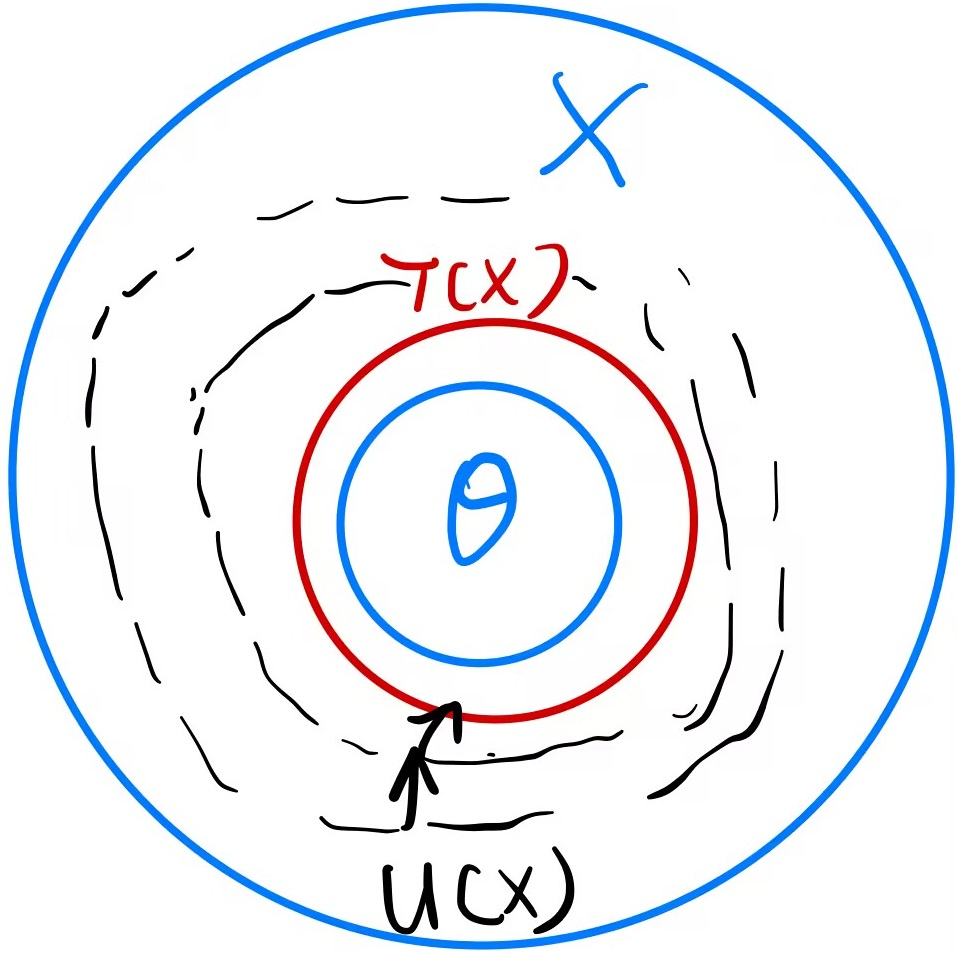
\includegraphics[width=0.41\textwidth]{./figures/chapter1/minimum_sufficient_statistic.png}
\end{figure}
\end{definition}

\begin{proposition}
$T(X),U(X)$ are the sufficient statistic, so
\begin{align*}
I(\theta;T(X)) &= I(\theta;X) \\
I(\theta;U(X)) &= I(\theta;X)
\end{align*}
$T(X)$ is the minimal sufficient statistic, so from data processing inequality:
$$I(X;T(X))\leq I(X;U(X))$$
understanding: 从上面的关系图来看, $T(X)$是对$U(X)$进行不断提纯,仅可能的去掉和$X$相关的信息, 只保留和$\theta$相关的信息.

e.g. 图像分类, 最理想的情况下, $(X,Y)$ 的最小充分统计量是$T(X)=Y$.
\end{proposition}
\section{Other codes*}
\begin{itemize}
\item Reed-Muller Code: 利用$\mathcal{C}$的线性性质.
\item Hudmard Code: 参数选择上有限制($n=2^m$)
\item LDPC Code(Low-Density Parity-Check Code) :5G中常用的编码方式, 逼近Shannon channel capacity
\end{itemize}
Details in PPT Lecture 4 Channle Encoding.
\chapter{Differential Entropy}

连续熵 / 微分熵. \qquad Book Chapter8. (P269)

nat(aka. nit / nepit) 是信息论中的单位, 将以 nat 为单位的量中所有的 $\ln$ 都换成 $\log$, 即可换算成单位 bit. $1 \text{ nat} = \ln e \text{ nat} = \log e \text{ bit} = \dfrac{1}{\ln 2} \text{ bit}$.

\section{Law of Large Numbers}

几种收敛方式:
Given a sequence $X_1,X_2,\ldots,X_n$, it converges to $X$:
\begin{itemize}
\item[1.] In probability(依概率收敛):
$$\lim\limits_{n\to\infty}P\left(|X_n-X|>\epsilon\right)=0\Rightarrow\lim\limits_{n\to\infty}P\left(|X_n-X|>\epsilon\right)<\delta$$
\item[2.] In mean square(均方收敛): $\lim\limits_{n\to\infty}\mathbb{E}\left[(X_n-X)^2\right]=0$.
\item[3.] Almost surely / with probability 1: $P\left(\lim\limits_{n\to\infty}X_n=X\right)=1$.
\end{itemize}

Law of Large Numbers(LLN): 大数定律.
$x_1,\ldots,x_n\stackrel{i.i.d.}{\sim}p(x)$, then $\dfrac{1}{n}\sum\limits_{i=1}^nx_i$ converges to $\mathbb{E}[x]$.

(1) in probability: Weak LLN(Weak Law of Large Numbers).

(2) w.p. $1$: Strong LLN(Strong Law of Large Numbers).
\section{Entropy Rates of Stochastic Processes}


\begin{definition}
The \textbf{entropy rate} of a stochastic process $\{X_i\}$ is defined as
$$H\left(\mathcal{X}\right) = \lim_{n\to\infty} \frac{1}{n}H(X_1,X_2,\cdots,X_n)$$
\end{definition}
随机过程$X(t)$的不确定度为$H(X(t))$, 整个随机过程的不确定度为$H\left(\mathcal{X}\right)$. $H\left(\mathcal{X}\right)$平衡整个过程中每个变量的不确定度(信息量), 极限可能不存在(e.g. 趋于极限时$H(\mathcal{X}$)可能在振荡, 而不是收敛到具体值).但$H\left(\mathcal{X}\right)$一定有界:
$$0\leq H(X_i)\leq \log|\mathcal{X}| \Rightarrow 0\leq H\left(\mathcal{X}\right)\leq \log|\mathcal{X}|$$

\begin{example}
\begin{itemize}
\item[1.] $X_1,X_2,\cdots,X_n$ are i.i.d., then:
$$H\left(\mathcal{X}\right) = \lim_{n\to\infty} \dfrac{1}{n}H(X_1,X_2,\cdots,X_n) = \lim_{n\to\infty} \dfrac{1}{n}\sum_{i=1}^nH(X_i) = H(X_1) = \ldots = H(X_n)$$

\item[2.] $X_1\perp X_2\perp\ldots\perp X_n$, then:
$$H\left(\mathcal{X}\right)=\lim_{n\to\infty}\dfrac{1}{n}H(X_1,X_2,\cdots,X_n) = \lim_{n\to\infty}\dfrac{1}{n}\sum_{i=1}^nH(X_i)$$

\end{itemize}
\end{example}

\begin{definition}
Define a related quantity for entropy rate:
$$H'\left(\mathcal{X}\right) = \lim_{n\to\infty}H(X_n|X_{n-1},X_{n-2},\cdots,X_1)$$
\end{definition}

\begin{theorem}
For a stationary stochastic process $\{X(t)\}$, $H\left(\mathcal{X}\right)$ limit exists:
$$H\left(\mathcal{X}\right) = H'\left(\mathcal{X}\right) = \lim_{n\to\infty}H(X_n|X_{n-1},X_{n-2},\cdots,X_1)$$
\end{theorem}

\begin{example}
For a stationary Markov chain: $X_1\rightarrow X_2\rightarrow\cdots\rightarrow X_n$ \textbf{(记忆为1!)}
$$H\left(\mathcal{X}\right)=H'\left(\mathcal{X}\right)=\lim_{n\to\infty}H(X_n|X_{n-1},\ldots,X_1)=H(X_n|X_{n-1})=\ldots=H(X_2|X_1)$$
\end{example}
\section{Fano's Inequality, Channel Coding Theorem(Shannon's Second Theorem)}
简单理解: 从jointly typical set的角度. 在第四章的最后(jointly AEP), 每个$X^n$平均会有$\frac{2^{nH(X,Y)}}{2^{nH(X)}}=2^{nH(Y|X)}$个$Y^n$与之jointly typical, 即将所有的$Y^n$进行划分, 每份的大小为$2^{nH(Y|X)}$, 可以分成 $\frac{2^{nH(Y)}}{2^{nH(Y|X)}}=2^{nI(X;Y)}$份. 这样平均每次用信道发送的bit数为$\frac{2^{nI(X;Y)}}{n}=I(X;Y)$

在保证无损传输的情况下, 信道容量:
$$C\triangleq\max R=\max\limits_{p(x)}I(X;Y)$$

\begin{definition}
Channel Coding Theorem(Shannon's Second Theorem) \\
对于一个rate 为 $R$ 的DMC, 只要$R<C$, 那么这个DMC是 \textcolor{blue}{achievable} 的. i.e. $\forall R<C, \exists$ a sequence of $\left(2^{nR},n\right)$ codes, 使得最大错误概率$\lambda^{(n)}\to 0$. \\
\textcolor{blue}{Conversely}, 任意sequence of $\left(2^{nR},n\right)$ codes, $\lambda^{(n)}\to 0$, 那么$R\leq C$.
\end{definition}
所以证明需要从两个角度: \\
1. 可达性证明(\textcolor{blue}{achievable} proof): $\forall R<C$, $\exists (R,n)$, s.t. $\lambda^{(n)}\to 0$, 找到一种达到$C$的方法. \\
2. \textcolor{blue}{converse} proof: 所有方法都不可能超过$C$. i.e. $R>C$时, $p_e^{(n)}\to 1 \Rightarrow R\leq C$时, $p_e^{(n)}\not\to 0$.


\textcolor{blue}{1. 可达性证明 achievable proof}:

<1>. 码本构建(randomly coding): fixed $p(x)$, 产生$2^{nR}$个长度为$n$的codewords: $X^n(1),\ldots,X^n(2^{nR})\stackrel{i.i.d.}{\sim}p(X^n)=\prod\limits_{i=1}^np(x_i)$.
\begin{figure}[htbp]
    \centering
    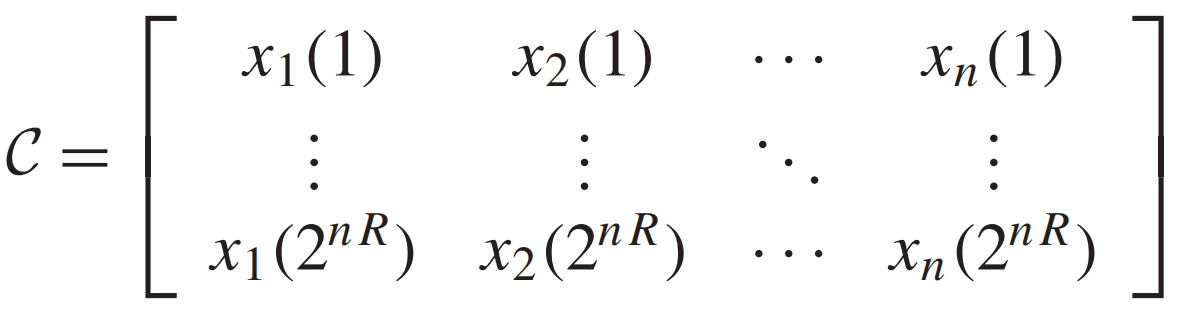
\includegraphics[width=0.5\textwidth]{./figures/chapter5/codebook.png}
\end{figure}

$X_i(w)$表示第$w$个codeword的第$i$个bit(下标为$i$). \\
码本构建好之后发给发送端和接收端(is known by the encoder and the decoder). 同时, 认为sender和receiver知道channel transition matrix $p(y|x)$.

<2>. Encoder: 随机生成一个数字 $w$, $p(W=w)=\dfrac{1}{2^{nR}}$, 从codebook $\mathcal{C}$中找出第$w$行$X^n(w)$, 发到信道当中.

<3> Decoder: reciver 接收由 $p(y^n|x^n(w))=\prod\limits_{i=1}^np(y_i|x_i(w))$ 生成的 $y^n$, 从codebook中找出一条message $\hat{W}$, s.t. $(X^n(\hat{W}), y^n)\in A_{\epsilon}^{(n)}(P_{X,Y})$, 且 no other index $W'\neq \hat{W}$ s.t. $(X^n(W'), y^n)\in A_{\epsilon}^{(n)}(P_{X,Y})$.

若找不到$\hat{W}$, an error is decleared.

<4> Error probability analysis: \\
先忽略码本的随机性 ($p(\mathcal{C})=\prod\limits_{w}^{2^{nR}}\prod\limits_{i=1}^np(x_i)(w)$), 考虑单一码本的情况. \\
发生错误: $\mathcal{E}=\left\{\hat{W}(Y^n) \neq W\right\}$. \\
考虑定义: $\lambda(i)=\Pr\left[\hat{W}\neq i|W=i\right]$, 则 $\Pr\left[\mathcal{E}|W=i\right]=\lambda(i)$. \\
$\Rightarrow \Pr\left[\hat{W}\neq W\right]=\sum\limits_{w=1}^{2^{nR}}p(W=w)\lambda(w)=\sum\limits_{w=1}^{2^{nR}}\dfrac{1}{2^{nR}}\lambda(w)$.

由于$W=1,\ldots,2^{nR}$是等概率产生的, 且地位相同, 所以 W.L.O.G. 取 $W=1$时的情况进行分析:

定义事件 $E_i=\left\{\left(X^{n}(i),Y^n\right)\in A_{\epsilon}^{(n)}(P_{X,Y})\right\}$, i.e. the i-th codeword is joint typical with the received sequence $Y^n$. \\
由jointly AEP, we can get that for sufficiently large $n$:
$$\Pr\left[E_1^c:\left(X^{n}(i),Y^n\right)\not\in A_{\epsilon}^{(n)}(P_{X,Y}) \right]\to 0 \Rightarrow \Pr\left[E_1^c: \left(X^{n}(i),Y^n\right)\not\in A_{\epsilon}^{(n)}(P_{X,Y})\right]\leq \epsilon$$
由于生成codebook $\mathcal{C}$时, 每一行的产生是独立的, i.e. $X^n(1)$与$X^n(2),\ldots,X^n(2^{nR})$是独立的, 所以$Y^n$与$X^n(i)$也是独立的, 所以有:
$$\Pr\left[E_i:\left(X^{n}(i),Y^n\right)\in A_{\epsilon}^{(n)}(P_{X,Y}) \right]\leq 2^{-n\left(I(X;Y)-3\epsilon\right)}$$
由jointly AEP, 当$R<I(X;Y)-3\epsilon$时
\begin{align*}
\Pr\left[\hat{W}\neq 1|W=1\right] &= \Pr\left[E_1^c\cup E_2\cup\ldots\cup E_{2^{nR}}\right] \\
&\leq \Pr\left[E_1^c\right] + \sum\limits_{w=2}^{2^{nR}}\Pr\left[E_w\right] \\
&\leq \epsilon + (2^{nR}-1) 2^{-n\left(I(X;Y)-3\epsilon\right)} \\
&\leq \epsilon + 2^{n\left(R-I(X;Y)+3\epsilon\right)} \\
&\leq 2\epsilon \quad \text{(sufficiently large $n$, $R<I(X;Y)-3\epsilon\Rightarrow 2^{n\left(R-I(X;Y)+3\epsilon\right)}\to 0<\epsilon$)}
\end{align*}
总结: 选择证明中取等时的分布作为真实分布 $p(x)\gets p^*(x)$, 此时$\forall R<I(X;Y)-3\epsilon$, i.e. $R<C$, 错误概率$p_e^{(n)}=\Pr\left[\hat{W}\neq W\right]\to 0\Rightarrow \lambda^{(n)}\to 0$. (Actually, $\lambda^{(n)}$条件比$p_e^{(n)}$更强, 但是$p_e^{(n)}$更容易计算)

若将codebook $\mathcal{C}$ 的随机性也考虑进去, 则会得到更加平均的结果:
$$\Pr\left[\hat{W}\neq W\right]=\sum_{w=1}^{2^{nR}}\sum_{\mathcal{C}}\Pr[\mathcal{C}]\dfrac{1}{2^{nR}}\lambda_w(\mathcal{C})=\lambda_1(\mathcal{C})\Rightarrow \Pr(\mathcal{E}|\mathcal{C}^*)\leq 2\epsilon$$
The best codebook $\mathcal{C}^*$ 中必然由超过一半的indices $i$ and their assciated codewords $X^n(i)$, 满足 $\lambda_i\leq 4\epsilon$, 否则$\Pr(\mathcal{E}|\mathcal{C}^*)>2\epsilon$. 砍去另一半codewords, 可以得到rate为$R'=\dfrac{\frac{2^{nR}}{2}}{n}=R-\dfrac{1}{n}$, s.t. $\lambda^{(n)}\leq 4\epsilon\to 0$. 所以可以使得 $\epsilon$ 不断的取小, 说明了$R$可以取到$C$的任意接近的地方.(取$p^*(x)$时, $C=I(X;Y), R=I(X;Y)-3\epsilon\to C$)

由此证明了 Achievability.

\begin{proposition}
Zero-error codes.
$$p_e^{(n)}\to 0 \Rightarrow R\leq C$$
\end{proposition}
proof: \\
Channel encoding 满足Markov chain $W\to X^n(W)\to Y^n\to \hat{W}$, so from data-processing inequality:
$$I(W; Y^n)\leq I(X^n(W); Y^n)$$

由 DMC的 memoryless, i.e. $p(Y_i|Y_1,\ldots,Y_{i-1},X^n)=p(Y_i|X_i)$, so
\begin{align*}
I(X^n;Y^n) &= H(Y^n) - H(Y^n|X^n) \\
&= \sum_{i=1}^nH(Y_i|Y_1,\ldots,Y_{i-1}) - \sum_{i=1}^nH(Y_i|Y_1,\ldots,Y_{i-1}, X^n) \\
&\leq \sum_{i=1}^nH(Y_i) - \sum_{i=1}^nH(Y_i|X_i) \qquad \text{(memoryless \& conditioning reduced entropy)} \\
&= \sum_{i=1}^n I(X_i;Y_i) \\
&\leq nC \qquad\qquad\qquad\qquad\qquad\quad\ \ \text{($Y_i$ are independent, $p_i(x)=p^*(x)$)}
\end{align*}

Since the channel is zero-error, so $\hat{W}=g(Y^n)=W$, i.e. $H(W|Y^n)=0$.
\begin{align*}
nR &= H(W) \\
&= H(W|Y^n) + I(W;Y^n) \\
&= I(W;Y^n) \qquad\quad\ \text{($H(W|Y^n)=0$)} \\
&\leq I(X^n;Y^n) \qquad\quad \text{(data-processing inequality)} \\
&\leq nC
\end{align*}

So for any zero-error $\left(2^{nR}, n\right)$ code, for all $n$:
$$R\leq C$$

\textcolor{blue}{2. converse proof: 证明$R>C$时, $p_e^{(n)}\to 1$ or $p_e^{(n)}\not\to 0$ as $n\to\infty$.}

\begin{definition}
Fano's Inequality: 是关于$p_e$的函数, 建立条件熵和错误概率$p_e$的关系. \\
For any estimator $\hat{X}$ such that $X\to Y\to \hat{X}$, $p_e=P(\hat{X}\neq X)$, then
$$H(p_e)+p_e\log\left|\mathcal{X}\right|\geq H(X|\hat{X})\geq H(X|Y)$$
It could be weakened to:
$$1+p_e\log\left|\mathcal{X}\right|\geq H(X|\hat{X})\geq H(X|Y)$$
or
$$p_e\geq \frac{H(X|Y)-1}{\log\left|\mathcal{X}\right|}$$
\end{definition}

Proof: \\
Let $E$ be the auxiliary variable indicate where the prediction is correct. i.e.
$$E=\begin{cases}
    1, & \text{if } \hat{X}\neq X \\
    0, & \text{if } \hat{X}=X
\end{cases}$$
Then we have $p(E=1)=p_e$, so
\begin{align*}
H\left(E,X|\hat{X}\right) &= \underbrace{H\left(E|\hat{X}\right)}_{\leq H(p_e)}+\underbrace{H\left(X|E,\hat{X}\right)}_{\leq p_e\log\left|\mathcal{X}\right|} \\
&= H\left(X|\hat{X}\right)+\underbrace{H\left(E|X,\hat{X}\right)}_{=0}
\end{align*}
其中由于$E=\mathbb{I}_{X=\hat{X}}$, 所以$H\left(E|X,\hat{X}\right)=0$. \\
由于conditioning reduces entropy, 所以 $H\left(E|\hat{X}\right)\leq H(E)=H(p_e)$. \\
同时有当$E=1$时, 给定$\hat{X}$, $X$的取值共有$\left|\mathcal{X}\right|-1$种, 所以有:
\begin{align*}
H\left(X|E, \hat{X}\right) &= \sum_{e=0,1}H\left(X|E=e, \hat{X}\right)P(E=e) \\
&\leq p_e\log\left(\left|\mathcal{X}\right|-1\right) + (1-p_e)\cdot 0 \\
&\leq p_e\log\left|\mathcal{X}\right|
\end{align*}
综上, 可以得到 Fano's Inequality:
$$H(p_e)+p_e\log\left|\mathcal{X}\right|\geq H(X|\hat{X})$$
weakened to的版本可由$H\left(p_e\right)\leq 1$, 以及数据处理不等式得到:
$$I(X;Y)\geq I(X;\hat{X})\Rightarrow H(X)-H(X|Y)\geq H(X)-H(X|\hat{X})\Rightarrow H(X|\hat{X})\geq H(X|Y)$$

由于 Channel encoding 满足Markov chain $W\to X^n(W)\to Y^n\to \hat{W}$, 所以应用Fano's Inequality:
$$H(W|\hat{W})\leq H(p_e^{(n)})+p_e^{(n)}\log\left|\mathcal{W}\right|$$
其中$\mathcal{W}=\left\{1,\ldots,2^{nR}\right\}$, 所以 $\left|\mathcal{W}\right|=2^{nR}\Rightarrow \log\left|\mathcal{W}\right|=nR$, 由于$W$是等概率产生的, 所以$H(W)= \log\left|\mathcal{W}\right| = nR$. 所以有
\begin{align*}
nR &= H(W) \\
&= H(W|\hat{W}) + I(W;\hat{W}) \qquad\qquad\quad \text{(definition of mutual information)} \\
&\leq H(p_e^{(n)})+p_e^{(n)} nR + I(W;\hat{W}) \qquad \text{(Fano's Inequality)} \\
&\leq 1 + p_e^{(n)}nR + nC \qquad \text{($I(W;\hat{W})\leq I(X^n;Y^n)\leq nC$ proved in zero-error code part)} \\
\Rightarrow R &\leq \dfrac{1}{n} + p_e^{(n)}R + C \\
\Rightarrow p_e^{(n)} &\geq 1 - \dfrac{C}{R} - \dfrac{1}{nR}
\end{align*}

取等条件: $W,\hat{W}$ 无信息丢失(zero-error code), i.e. $X^n=f(W), Y^n=g(X^n)$是$W$的充分统计量, $W$到$\hat{W}$是一对一的映射. 由充分统计量(s.s.), 此时可以看作构成 Markov Chain:
\begin{align*}
W \to X^n \to Y^n \to \hat{W} \\
W \to \hat{W} \to X^n \to Y^n
\end{align*}

由于我们的前提假设是 $R>C$, 且 $R,C$ 为常数, 所以 $\dfrac{C}{R}<1$, 是常数. 当$n\to\infty$时, $\dfrac{1}{nR}\to 0<\epsilon$, 所以 $p_e^{(n)}\geq 1-\text{(constant less than $1$)} - \epsilon \not\to 0$.

所以我们证明了 $\forall R>C, p_e^{(n)}\not\to 0$, 即证明了converse proof.
\chapter{Gaussian Channel}

Book Chapter9. (P287)

连续信号, 高斯信道的信道容量为 $C = \dfrac{1}{2} \log\left(1+\dfrac{P}{N}\right)$. 这是无线通讯领域内的重要结论. 这里的 $\dfrac{P}{N}$ 是信噪比, i.e. Signal to Noise Ratio (SNR).

\section{Law of Large Numbers}

几种收敛方式:
Given a sequence $X_1,X_2,\ldots,X_n$, it converges to $X$:
\begin{itemize}
\item[1.] In probability(依概率收敛):
$$\lim\limits_{n\to\infty}P\left(|X_n-X|>\epsilon\right)=0\Rightarrow\lim\limits_{n\to\infty}P\left(|X_n-X|>\epsilon\right)<\delta$$
\item[2.] In mean square(均方收敛): $\lim\limits_{n\to\infty}\mathbb{E}\left[(X_n-X)^2\right]=0$.
\item[3.] Almost surely / with probability 1: $P\left(\lim\limits_{n\to\infty}X_n=X\right)=1$.
\end{itemize}

Law of Large Numbers(LLN): 大数定律.
$x_1,\ldots,x_n\stackrel{i.i.d.}{\sim}p(x)$, then $\dfrac{1}{n}\sum\limits_{i=1}^nx_i$ converges to $\mathbb{E}[x]$.

(1) in probability: Weak LLN(Weak Law of Large Numbers).

(2) w.p. $1$: Strong LLN(Strong Law of Large Numbers).
\section{Entropy Rates of Stochastic Processes}


\begin{definition}
The \textbf{entropy rate} of a stochastic process $\{X_i\}$ is defined as
$$H\left(\mathcal{X}\right) = \lim_{n\to\infty} \frac{1}{n}H(X_1,X_2,\cdots,X_n)$$
\end{definition}
随机过程$X(t)$的不确定度为$H(X(t))$, 整个随机过程的不确定度为$H\left(\mathcal{X}\right)$. $H\left(\mathcal{X}\right)$平衡整个过程中每个变量的不确定度(信息量), 极限可能不存在(e.g. 趋于极限时$H(\mathcal{X}$)可能在振荡, 而不是收敛到具体值).但$H\left(\mathcal{X}\right)$一定有界:
$$0\leq H(X_i)\leq \log|\mathcal{X}| \Rightarrow 0\leq H\left(\mathcal{X}\right)\leq \log|\mathcal{X}|$$

\begin{example}
\begin{itemize}
\item[1.] $X_1,X_2,\cdots,X_n$ are i.i.d., then:
$$H\left(\mathcal{X}\right) = \lim_{n\to\infty} \dfrac{1}{n}H(X_1,X_2,\cdots,X_n) = \lim_{n\to\infty} \dfrac{1}{n}\sum_{i=1}^nH(X_i) = H(X_1) = \ldots = H(X_n)$$

\item[2.] $X_1\perp X_2\perp\ldots\perp X_n$, then:
$$H\left(\mathcal{X}\right)=\lim_{n\to\infty}\dfrac{1}{n}H(X_1,X_2,\cdots,X_n) = \lim_{n\to\infty}\dfrac{1}{n}\sum_{i=1}^nH(X_i)$$

\end{itemize}
\end{example}

\begin{definition}
Define a related quantity for entropy rate:
$$H'\left(\mathcal{X}\right) = \lim_{n\to\infty}H(X_n|X_{n-1},X_{n-2},\cdots,X_1)$$
\end{definition}

\begin{theorem}
For a stationary stochastic process $\{X(t)\}$, $H\left(\mathcal{X}\right)$ limit exists:
$$H\left(\mathcal{X}\right) = H'\left(\mathcal{X}\right) = \lim_{n\to\infty}H(X_n|X_{n-1},X_{n-2},\cdots,X_1)$$
\end{theorem}

\begin{example}
For a stationary Markov chain: $X_1\rightarrow X_2\rightarrow\cdots\rightarrow X_n$ \textbf{(记忆为1!)}
$$H\left(\mathcal{X}\right)=H'\left(\mathcal{X}\right)=\lim_{n\to\infty}H(X_n|X_{n-1},\ldots,X_1)=H(X_n|X_{n-1})=\ldots=H(X_2|X_1)$$
\end{example}
\chapter{Rate Distortion Theory*}

Book Chapter10. (P327)

率失真理论

\section{Law of Large Numbers}

几种收敛方式:
Given a sequence $X_1,X_2,\ldots,X_n$, it converges to $X$:
\begin{itemize}
\item[1.] In probability(依概率收敛):
$$\lim\limits_{n\to\infty}P\left(|X_n-X|>\epsilon\right)=0\Rightarrow\lim\limits_{n\to\infty}P\left(|X_n-X|>\epsilon\right)<\delta$$
\item[2.] In mean square(均方收敛): $\lim\limits_{n\to\infty}\mathbb{E}\left[(X_n-X)^2\right]=0$.
\item[3.] Almost surely / with probability 1: $P\left(\lim\limits_{n\to\infty}X_n=X\right)=1$.
\end{itemize}

Law of Large Numbers(LLN): 大数定律.
$x_1,\ldots,x_n\stackrel{i.i.d.}{\sim}p(x)$, then $\dfrac{1}{n}\sum\limits_{i=1}^nx_i$ converges to $\mathbb{E}[x]$.

(1) in probability: Weak LLN(Weak Law of Large Numbers).

(2) w.p. $1$: Strong LLN(Strong Law of Large Numbers).
\section{Entropy Rates of Stochastic Processes}


\begin{definition}
The \textbf{entropy rate} of a stochastic process $\{X_i\}$ is defined as
$$H\left(\mathcal{X}\right) = \lim_{n\to\infty} \frac{1}{n}H(X_1,X_2,\cdots,X_n)$$
\end{definition}
随机过程$X(t)$的不确定度为$H(X(t))$, 整个随机过程的不确定度为$H\left(\mathcal{X}\right)$. $H\left(\mathcal{X}\right)$平衡整个过程中每个变量的不确定度(信息量), 极限可能不存在(e.g. 趋于极限时$H(\mathcal{X}$)可能在振荡, 而不是收敛到具体值).但$H\left(\mathcal{X}\right)$一定有界:
$$0\leq H(X_i)\leq \log|\mathcal{X}| \Rightarrow 0\leq H\left(\mathcal{X}\right)\leq \log|\mathcal{X}|$$

\begin{example}
\begin{itemize}
\item[1.] $X_1,X_2,\cdots,X_n$ are i.i.d., then:
$$H\left(\mathcal{X}\right) = \lim_{n\to\infty} \dfrac{1}{n}H(X_1,X_2,\cdots,X_n) = \lim_{n\to\infty} \dfrac{1}{n}\sum_{i=1}^nH(X_i) = H(X_1) = \ldots = H(X_n)$$

\item[2.] $X_1\perp X_2\perp\ldots\perp X_n$, then:
$$H\left(\mathcal{X}\right)=\lim_{n\to\infty}\dfrac{1}{n}H(X_1,X_2,\cdots,X_n) = \lim_{n\to\infty}\dfrac{1}{n}\sum_{i=1}^nH(X_i)$$

\end{itemize}
\end{example}

\begin{definition}
Define a related quantity for entropy rate:
$$H'\left(\mathcal{X}\right) = \lim_{n\to\infty}H(X_n|X_{n-1},X_{n-2},\cdots,X_1)$$
\end{definition}

\begin{theorem}
For a stationary stochastic process $\{X(t)\}$, $H\left(\mathcal{X}\right)$ limit exists:
$$H\left(\mathcal{X}\right) = H'\left(\mathcal{X}\right) = \lim_{n\to\infty}H(X_n|X_{n-1},X_{n-2},\cdots,X_1)$$
\end{theorem}

\begin{example}
For a stationary Markov chain: $X_1\rightarrow X_2\rightarrow\cdots\rightarrow X_n$ \textbf{(记忆为1!)}
$$H\left(\mathcal{X}\right)=H'\left(\mathcal{X}\right)=\lim_{n\to\infty}H(X_n|X_{n-1},\ldots,X_1)=H(X_n|X_{n-1})=\ldots=H(X_2|X_1)$$
\end{example}
\chapter{Information Bottleneck*}
\begin{figure}[htbp]
    \centering
    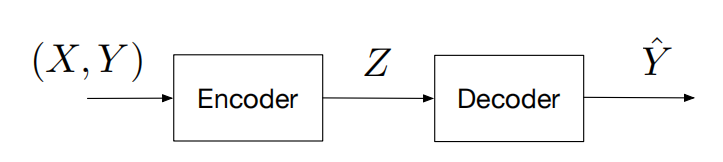
\includegraphics[width=0.8\textwidth]{./figures/chapter9/AE.png}
\end{figure}
$(X, Y)$: Source input, $Z$: extracted features, $\hat{Y}$: predicted label. \\
Information complexity: $I(X;Z)$, information utility: $I(Z;Y)$. \\
Trade-off: $L = \min\limits_{p(z|x)} I(X;Z) - \beta I(Z;Y)$, 其中后半部分是为了防止过拟合.

\begin{figure}[htbp]
    \centering
    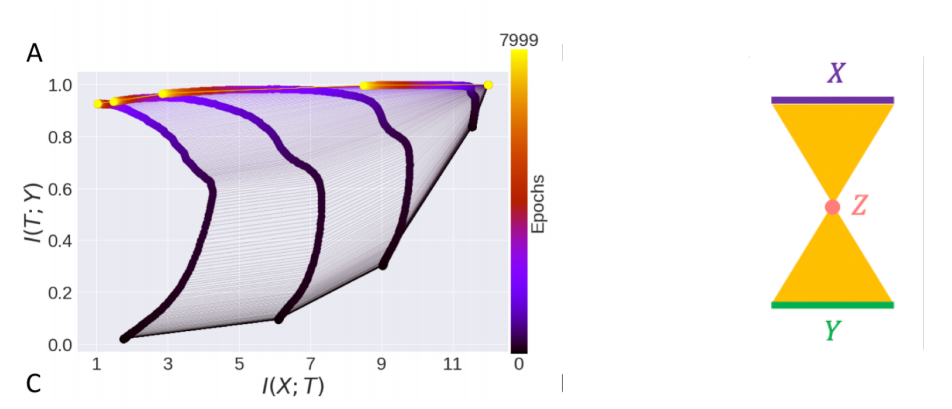
\includegraphics[width=0.8\textwidth]{./figures/chapter9/bottleneck.png}
\end{figure}
若将 Encoder 和 Decoder 都换成 neural network, 则会出现上图的现象. \\
从左往右四条线是网络的深度, 在同一层中, 互信息会先增大后降低. 感性理解: 学习的过程中需要先把书学厚, 然后再学薄.

\begin{figure}[htbp]
    \centering
    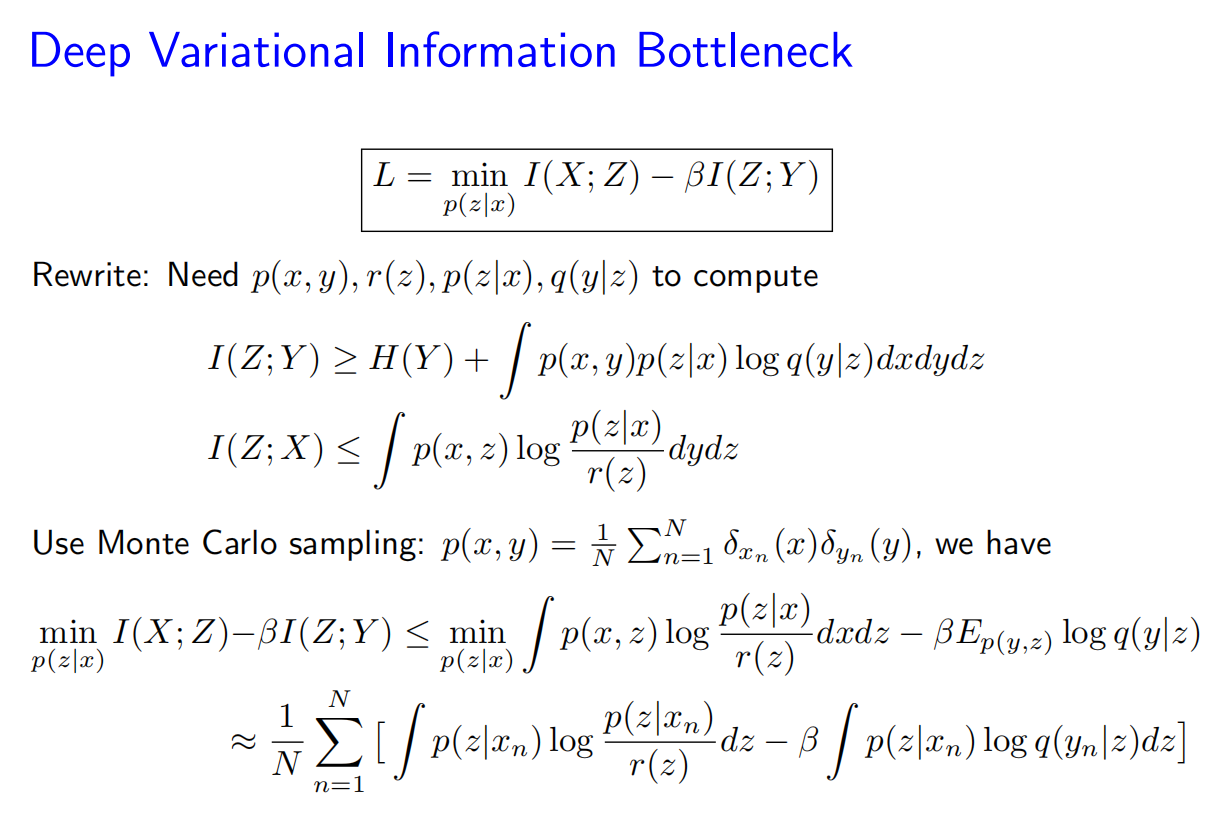
\includegraphics[width=\textwidth]{./figures/chapter9/result.png}
\end{figure}
$p(z|x)$为训练得到的encoder, $p(y|z)$为训练得到的decoder. $p(x,y)$ 无法直接得到, 用 Monte Carlo从样本中采样估计. \\
VAE中重参数化, ELBO等 details in PPT.

\chapter{Appendix}

\section{Axiomatic definition of entropy}
\label{sec:Axiomatic_definition_of_entropy}
熵的公理定义

If we assume certain axioms for our measure of information, we will be forced to use a logarithmic measure such as entropy. Shannon used this to justify his initial definition of entropy.

If a sequence of symmetric functions $H_m\left(p_1, p_2, \ldots, p_m\right)$ satisfies the following properties: \\
1. Normalization: $H_2\left(\dfrac{1}{2}, \dfrac{1}{2}\right)=1$ \\
2. Continuity: $H_2(p, 1-p)$ is a continuous function of $p$ \\
3. Grouping: $H_m\left(p_1, p_2, \ldots, p_m\right)=H_{m-1}\left(p_1+p_2, p_3, \ldots, p_m\right)+$ $\left(p_1+p_2\right) H_2\left(\dfrac{p_1}{p_1+p_2}, \dfrac{p_2}{p_1+p_2}\right)$

prove that $H_m$ must be of the form
$$H_m\left(p_1, p_2, \ldots, p_m\right)=-\sum_{i=1}^m p_i \log p_i, \quad m=2,3, \ldots$$

\textcolor{blue}{Solution}

Notations:
\begin{align*}
f(m) &\triangleq H_m\left(\dfrac{1}{m}, \dfrac{1}{m}, \ldots, \dfrac{1}{m}\right) \\
S_k &\triangleq \sum_{i=1}^k p_i \quad k=1,2,\ldots,m
\end{align*}

From the grouping property, we can get its extension:
\begin{align*}
&\quad H_m\left(p_1,p_2, p_3, \ldots, p_m\right) \\
&= H_{m-1}\left(S_2, p_3, \ldots, p_m\right)+S_2 H_2\left(\dfrac{p_1}{S_2}, \dfrac{p_2}{S_2}\right) \\
&= H_{m-2}\left(S_3, p_4, \ldots, p_m\right)+S_3 H_2\left(\dfrac{p_1+p_2}{S_3}, \dfrac{p_3}{S_3}\right)+S_2 H_2\left(\dfrac{p_1}{S_2}, \dfrac{p_2}{S_2}\right) \\
&= \ldots \\
&= \textcolor{blue}{H_{m-(k-1)}(S_k, p_{k+1}, \ldots, p_m)+\sum_{i=2}^k S_iH_2\left(\dfrac{S_{i-1}}{S_i}, \dfrac{p_i}{S_i}\right)} \\
&= \textcolor{blue}{H_{m-(k-1)}\left(S_{k}, p_{k+1}, \ldots, p_m\right) + S_kH_k\left(\dfrac{p_1}{S_k}, \dfrac{p_2}{S_k}, \ldots, \dfrac{p_{k}}{S_k}\right)}
\end{align*}
The last equality(\textcolor{blue}{blue part}) can be obtained by expanding $H_k\left(\dfrac{p_1}{S_k}, \dfrac{p_2}{S_k}, \ldots, \dfrac{p_{k}}{S_k}\right)$.

And using this, we can get that
\begin{align*}
f(mn) &= H_{mn}\left(\dfrac{1}{mn}, \dfrac{1}{mn}, \ldots, \dfrac{1}{mn}\right) \\
&= H_{mn-(n-1)}\left(S_n, \dfrac{1}{mn}, \ldots, \dfrac{1}{mn}\right)+S_n H_n\left(\dfrac{1}{n}, \dfrac{1}{n}, \ldots, \dfrac{1}{n}\right) \\
&= H_{mn-2(n-1)}\left(S_n, S_n, \dfrac{1}{mn}, \ldots, \dfrac{1}{mn}\right)+2 S_n H_n\left(\dfrac{1}{n}, \dfrac{1}{n}, \ldots, \dfrac{1}{n}\right) \\
&= \ldots \\
&= H_{mn-m(n-1)}\left(S_n, S_n, \ldots, S_n\right)+m S_n H_n\left(\dfrac{1}{n}, \dfrac{1}{n}, \ldots, \dfrac{1}{n}\right) \\
&= H_m\left(\dfrac{1}{m}, \ldots, \dfrac{1}{m}\right) + m \dfrac{1}{m} H_n\left(\dfrac{1}{n}, \dfrac{1}{n}, \ldots, \dfrac{1}{n}\right) \\
&= f(m) + f(n)
\end{align*}

And since we have the Continuity property, i.e. $H_2(p, 1-p)$ is a continuous function of $p$, from the property and provement of Cauchy function, we could get that
$$f(m) = \log_a m$$

And from the Normalization property, we have
$$f(2) = 1$$
So we can get that $a=2$.

So above all, we have proved that
$$\textcolor{blue}{f(m)=H_m\left(\dfrac{1}{m}, \dfrac{1}{m}, \ldots, \dfrac{1}{m}\right)= \log_2 m}$$

And then prove $H_2(p,1-p) = -p\log_2p - (1-p)\log_2(1-p)$: \\
1. When $p$ is rational, suppose $p = \dfrac{r}{s}$, where $r,s$ are integers, $s>1,0\leq r\leq s$, $\gcd(r,s)=1$. Then from the Grouping property and its extension, we have:
\begin{align*}
f(s) &= H_s\left(\dfrac{1}{s},\ldots,\dfrac{1}{s}\right) = H_{s}\left(\underbrace{\dfrac{1}{s},\ldots,\dfrac{1}{s}}_r,\underbrace{\dfrac{1}{s},\ldots,\dfrac{1}{s}}_{s-r}\right) \\
&= H_{s-(r-1)}\left(\dfrac{r}{s},\underbrace{\dfrac{1}{s},\ldots,\dfrac{1}{s}}_{s-r}\right)+\dfrac{r}{s}H_r\left(\dfrac{1}{r},\ldots,\dfrac{1}{r}\right) \\
&= H_{s-(r-1)-(s-1)}\left(\dfrac{r}{s},\dfrac{s-r}{s}\right) + \dfrac{s-r}{s}H_{s-r}\left(\dfrac{1}{s-r},\ldots,\dfrac{1}{s-r}\right) + \dfrac{r}{s}H_r\left(\dfrac{1}{r},\ldots,\dfrac{1}{r}\right) \\
&= H_2(\dfrac{r}{s},\dfrac{s-r}{s}) + \dfrac{s-r}{s}f(s-r) + \dfrac{r}{s}f(r)
\end{align*}

And since $p=\dfrac{r}{s}$, so we can get that
\begin{align*}
H_2(p,1-p) &= H_2(\dfrac{r}{s},\dfrac{s-r}{s}) \\
&= f(s) -\dfrac{s-r}{s}f(s-r) - \dfrac{r}{s}f(r) \\
&= \log_2 s - (1-p)\log_2\left(s(1-p)\right) - p\log_2(sp) \\
&= -p\log_2p - (1-p)\log_2(1-p)
\end{align*}

2. When $p$ is irrational, since we have the Continuity property, so we can also get that
$$H_2(p,1-p) = -p\log_2p - (1-p)\log_2(1-p)$$

So above all, we have prove that $\forall p\in[0,1]$, we have
$$\textcolor{blue}{H_2(p,1-p) = -p\log_2p - (1-p)\log_2(1-p)}$$

Then we use the induction to prove that, suppose that
$$H_k(p_1, p_2, \ldots, p_k)=-\sum_{i=1}^k p_i \log p_i, \forall k=1,2,\ldots,m$$
Then for $k=m+1$, we have
\begin{align*}
H_k(p_1, p_2, \ldots, p_k) &= H_{m+1}(p_1, p_2, \ldots, p_{m+1}) \\
&= H_{m}(p_1+p_2, p_3, \ldots, p_{m+1}) + (p_1+p_2)H_2\left(\dfrac{p_1}{p_1+p_2}, \dfrac{p_2}{p_1+p_2}\right) \\
&= \left(-(p_1+p_2)\log(p_1+p_2)-\sum_{i=3}^{m+1}p_i\log p_i\right) - (p_1+p_2)\left(\dfrac{p_1}{p_1+p_2}\log\dfrac{p_1}{p_1+p_2} + \dfrac{p_2}{p_1+p_2}\log\dfrac{p_2}{p_1+p_2}\right) \\
&= -(p_1+p_2)\log(p_1+p_2)-\sum_{i=3}^{m+1}p_i\log p_i - p_1\log p_1 - p_2\log p_2 + (p_1+p_2)(\dfrac{p_1}{p_1+p_2}+\dfrac{p_2}{p_1+p_2})\log(p_1+p_2) \\
&= -\sum_{i=1}^{m+1}p_i\log p_i \\
&= -\sum_{i=1}^k p_i \log p_i
\end{align*}
So we have proved that $\forall m$, we have
$$H_m(p_1,\ldots,p_m)=-\sum_{i=1}^mp_i\log p_i.$$

So above all, we have proved that \footnote{The proof above has referenced from A Rényi.Wahrscheinlichkeitsrechnung, mit einem Anhang über Informationstheorie. Veb Deutscher Verlag der Wissenschaften, Berlin, 1962.}
$$\textcolor{blue}{H_m\left(p_1, p_2, \ldots, p_m\right)=-\sum_{i=1}^m p_i \log p_i, \quad m=2,3, \ldots}$$
% -------------------- chapters --------------------

\end{document}